\documentclass[a4paper,12pt,twoside]{memoir}

% Castellano
\usepackage[spanish,es-tabla]{babel}
\selectlanguage{spanish}
\usepackage[utf8]{inputenc}
\usepackage[T1]{fontenc}
\usepackage{lmodern} % scalable font
\usepackage{microtype}
\usepackage{placeins}
\usepackage{eurosym} % Añade el símbolo del Euro.

\RequirePackage{booktabs}
\RequirePackage[table]{xcolor}
\RequirePackage{xtab}
\RequirePackage{multirow}

% Bibliografía bajo norma UNE-ISO 690:2013.
\usepackage[
  backend=biber,     % "Backend" que genera la bibliografía.
  style=iso-numeric, % Usa el método de referencias numéricas.
  autolang=other,    % Soporta múltiples lenguajes en la bibliografía.
  sortlocale=es_ES,  % Ordena la bibliografía usando el lenguaje indicado.
  bibencoding=UTF8   % Codificación de caracteres de los archivos .bib.
]{biblatex}

% Indica el archivo usado por la memoria.
\addbibresource{bibliografiaAnexos.bib}

% Links
\usepackage[colorlinks]{hyperref}
\hypersetup{
	allcolors = {red}
}

% Ecuaciones
\usepackage{amsmath}

% Rutas de fichero / paquete
\newcommand{\ruta}[1]{{\sffamily #1}}

% Párrafos
\nonzeroparskip


% Imagenes
\usepackage{graphicx}
\newcommand{\imagen}[2]{
	\begin{figure}[!h]
		\centering
		\includegraphics[width=0.9\textwidth]{#1}
		\caption{#2}\label{fig:#1}
	\end{figure}
	\FloatBarrier
}

\newcommand{\imagenflotante}[2]{
	\begin{figure}%[!h]
		\centering
		\includegraphics[width=0.9\textwidth]{#1}
		\caption{#2}\label{fig:#1}
	\end{figure}
}



% El comando \figura nos permite insertar figuras comodamente, y utilizando
% siempre el mismo formato. Los parametros son:
% 1 -> Porcentaje del ancho de página que ocupará la figura (de 0 a 1)
% 2 --> Fichero de la imagen
% 3 --> Texto a pie de imagen
% 4 --> Etiqueta (label) para referencias
% 5 --> Opciones que queramos pasarle al \includegraphics
% 6 --> Opciones de posicionamiento a pasarle a \begin{figure}
\newcommand{\figuraConPosicion}[6]{%
  \setlength{\anchoFloat}{#1\textwidth}%
  \addtolength{\anchoFloat}{-4\fboxsep}%
  \setlength{\anchoFigura}{\anchoFloat}%
  \begin{figure}[#6]
    \begin{center}%
      \Ovalbox{%
        \begin{minipage}{\anchoFloat}%
          \begin{center}%
            \includegraphics[width=\anchoFigura,#5]{#2}%
            \caption{#3}%
            \label{#4}%
          \end{center}%
        \end{minipage}
      }%
    \end{center}%
  \end{figure}%
}

%
% Comando para incluir imágenes en formato apaisado (sin marco).
\newcommand{\figuraApaisadaSinMarco}[5]{%
  \begin{figure}%
    \begin{center}%
    \includegraphics[angle=90,height=#1\textheight,#5]{#2}%
    \caption{#3}%
    \label{#4}%
    \end{center}%
  \end{figure}%
}
% Para las tablas
\newcommand{\otoprule}{\midrule [\heavyrulewidth]}
%
% Nuevo comando para tablas pequeñas (menos de una página).
\newcommand{\tablaSmall}[5]{%
 \begin{table}
  \begin{center}
   \rowcolors {2}{gray!35}{}
   \begin{tabular}{#2}
    \toprule
    #4
    \otoprule
    #5
    \bottomrule
   \end{tabular}
   \caption{#1}
   \label{tabla:#3}
  \end{center}
 \end{table}
}

%
%Para el float H de tablaSmallSinColores
\usepackage{float}

%
% Nuevo comando para tablas pequeñas (menos de una página).
\newcommand{\tablaSmallSinColores}[5]{%
 \begin{table}[H]
  \begin{center}
   \begin{tabular}{#2}
    \toprule
    #4
    \otoprule
    #5
    \bottomrule
   \end{tabular}
   \caption{#1}
   \label{tabla:#3}
  \end{center}
 \end{table}
}

\newcommand{\tablaApaisadaSmall}[5]{%
\begin{landscape}
  \begin{table}
   \begin{center}
    \rowcolors {2}{gray!35}{}
    \begin{tabular}{#2}
     \toprule
     #4
     \otoprule
     #5
     \bottomrule
    \end{tabular}
    \caption{#1}
    \label{tabla:#3}
   \end{center}
  \end{table}
\end{landscape}
}

%
% Nuevo comando para tablas grandes con cabecera y filas alternas coloreadas en gris.
\newcommand{\tabla}[6]{%
  \begin{center}
    \tablefirsthead{
      \toprule
      #5
      \otoprule
    }
    \tablehead{
      \multicolumn{#3}{l}{\small\sl continúa desde la página anterior}\\
      \toprule
      #5
      \otoprule
    }
    \tabletail{
      \hline
      \multicolumn{#3}{r}{\small\sl continúa en la página siguiente}\\
    }
    \tablelasttail{
      \hline
    }
    \bottomcaption{#1}
    \rowcolors {2}{gray!35}{}
    \begin{xtabular}{#2}
      #6
      \bottomrule
    \end{xtabular}
    \label{tabla:#4}
  \end{center}
}

%
% Nuevo comando para tablas grandes con cabecera.
\newcommand{\tablaSinColores}[6]{%
  \begin{center}
    \tablefirsthead{
      \toprule
      #5
      \otoprule
    }
    \tablehead{
      \multicolumn{#3}{l}{\small\sl continúa desde la página anterior}\\
      \toprule
      #5
      \otoprule
    }
    \tabletail{
      \hline
      \multicolumn{#3}{r}{\small\sl continúa en la página siguiente}\\
    }
    \tablelasttail{
      \hline
    }
    \bottomcaption{#1}
    \begin{xtabular}{#2}
      #6
      \bottomrule
    \end{xtabular}
    \label{tabla:#4}
  \end{center}
}

%
% Nuevo comando para tablas grandes sin cabecera.
\newcommand{\tablaSinCabecera}[5]{%
  \begin{center}
    \tablefirsthead{
      \toprule
    }
    \tablehead{
      \multicolumn{#3}{l}{\small\sl continúa desde la página anterior}\\
      \hline
    }
    \tabletail{
      \hline
      \multicolumn{#3}{r}{\small\sl continúa en la página siguiente}\\
    }
    \tablelasttail{
      \hline
    }
    \bottomcaption{#1}
  \begin{xtabular}{#2}
    #5
   \bottomrule
  \end{xtabular}
  \label{tabla:#4}
  \end{center}
}



\definecolor{cgoLight}{HTML}{EEEEEE}
\definecolor{cgoExtralight}{HTML}{FFFFFF}

%
% Nuevo comando para tablas grandes sin cabecera.
\newcommand{\tablaSinCabeceraConBandas}[5]{%
  \begin{center}
    \tablefirsthead{
      \toprule
    }
    \tablehead{
      \multicolumn{#3}{l}{\small\sl continúa desde la página anterior}\\
      \hline
    }
    \tabletail{
      \hline
      \multicolumn{#3}{r}{\small\sl continúa en la página siguiente}\\
    }
    \tablelasttail{
      \hline
    }
    \bottomcaption{#1}
    \rowcolors[]{1}{cgoExtralight}{cgoLight}

  \begin{xtabular}{#2}
    #5
   \bottomrule
  \end{xtabular}
  \label{tabla:#4}
  \end{center}
}




\graphicspath{ {./img/} }

% Capítulos
\chapterstyle{bianchi}
\newcommand{\capitulo}[2]{
	\setcounter{chapter}{#1}
	\setcounter{section}{0}
	\chapter*{#2}
	\addcontentsline{toc}{chapter}{#2}
	\markboth{#2}{#2}
}

% Apéndices
\renewcommand{\appendixname}{Apéndice}
\renewcommand*\cftappendixname{\appendixname}

\newcommand{\apendice}[1]{
	%\renewcommand{\thechapter}{A}
	\chapter{#1}
}

\renewcommand*\cftappendixname{\appendixname\ }

% Formato de portada
\makeatletter
\usepackage{xcolor}
\newcommand{\tutor}[1]{\def\@tutor{#1}}
\newcommand{\course}[1]{\def\@course{#1}}
\definecolor{cpardoBox}{HTML}{E6E6FF}
\def\maketitle{
  \null
  \thispagestyle{empty}
  % Cabecera ----------------
\noindent
\includegraphics[width=\textwidth]{cabecera}\vspace{1cm}%
  \vfill
  % Título proyecto y escudo informática ----------------
  \colorbox{cpardoBox}{%
    \begin{minipage}{.8\textwidth}
      \vspace{.5cm}\Large
      \begin{center}
      \textbf{TFM del Máster Universitario en Ingeniería Informática}\vspace{.6cm}\\
      \textbf{\LARGE\@title{}}
      \end{center}
      \vspace{.2cm}
    \end{minipage}

  }%
  \hfill\begin{minipage}{.20\textwidth}
    
\includegraphics[width=\textwidth]{escudoInfor}
  \end{minipage}
  \vfill
  % Datos de alumno, curso y tutores ------------------
  \begin{center}%
  {%
    \noindent\LARGE
    Presentado por \@author{}\\ 
    en Universidad de Burgos --- \@date{}\\
    Tutor: \@tutor{}\\
  }%
  \end{center}%
  \null
  \cleardoublepage
  }
\makeatother

% Comando para formatear palabras procedentes de otros
% lenguajes distintos del castellano.
% Estas palabras se pueden escribir en letra cursiva 
\newcommand{\extranjerismo}[1]{\textit{#1}}
% o con comillas si no se dispone de cursiva.
%\newcommand{\extranjerismo}[1]{"{#1}"}

% Comando para formatear los títulos de otras obras de creación.
\newcommand{\titulo}[1]{\textit{#1}}

% Expande la palabra Software
\newcommand{\Sw}{\extranjerismo{Software}}
% Expande la palabra software
\newcommand{\sw}{\extranjerismo{software}}
% Expande la palabra Hardware
\newcommand{\Hw}{\extranjerismo{Hardware}}
% Expande la palabra hardware
\newcommand{\hw}{\extranjerismo{hardware}}

% Muestra una imagen con su ancho ajustado en relación al ancho del texto.
%
% #1 Nombre del fichero con la imagen.
% #2 Texto para el pie de foto.
% #3 Opciones para \begin{figure}.
% #4 Porcentaje del ancho (de 0 a 1) al que ajustar la imagen.
\newcommand{\imagenancho}[4]{
  \begin{figure}[#3]
    \centering
    \includegraphics[width=#4\textwidth]{#1}
    \caption{#2}
    \label{fig:#1}
  \end{figure}
}

% Muestra una imagen con su alto ajustado en relación al alto del texto.
%
% #1 Nombre del fichero con la imagen.
% #2 Texto para el pie de foto.
% #3 Opciones para \begin{figure}.
% #4 Porcentaje del alto (de 0 a 1) al que ajustar la imagen.
\newcommand{\imagenalto}[4]{
  \begin{figure}[#3]
    \centering
    \includegraphics[height=#4\textheight]{#1}
    \caption{#2}
    \label{fig:#1}
  \end{figure}
}

% Datos de portada
\title{Comunicación TCP/IP con sistemas empotrados \\Documentación Técnica}
\author{RPC}
\tutor{AMG}
\date{\today}

\begin{document}

\maketitle



\cleardoublepage



%%%%%%%%%%%%%%%%%%%%%%%%%%%%%%%%%%%%%%%%%%%%%%%%%%%%%%%%%%%%%%%%%%%%%%%%%%%%%%%%%%%%%%%%



\frontmatter


\clearpage

% Indices
\tableofcontents

\clearpage

\listoffigures

\clearpage

\listoftables

\clearpage

\mainmatter

\appendix

\apendice{Plan de proyecto software}

\section{Introducción}

Existen dos temas a tratar en este apéndice. 
El primero corresponde a la planificación temporal del trabajo, en la cual veremos las tareas realizadas y los tiempos requeridos para llevarlas a cabo. También veremos el tiempo total necesario para la realización de este proyecto.  \\
El segundo tema que se va a desarrollar, es la realización de un análisis de la viabilidad de un proyecto de estas características en la vida real. Para ello nos centraremos en analizar las variables económicas y legales referentes al desarrollo de este trabajo. En cuanto a este último punto veremos los tipos de licencias que se pueden utilizar en este tipo de software


\section{Planificación temporal}

Como ya hemos comentado, la planificación del proyecto se llevó a cabo siguiendo la metodología SCRUM que está basada entre otras cosas, en el uso de \extranjerismo{sprints} para organizar la carga de tareas. 

Según esta metodología, estos sprints deben durar entre 1 y 3 semanas. Puesto que se está utilizando una metodología SCRUM, algunos tiempos pueden no ajustarse lo suficiente a lo esperado sobre todo los de los primeros sprint realizados, ya que en estos se debe llevar un proceso de medición de fuerzas y dificultades del trabajo a realizar. En este caso y puesto que mi situación personal ha sido distinta a lo largo de este proceso, la duración de estos sprints no ha sido siempre la misma. Esto se debe a que mis obligaciones han ido variando a medida que avanzaba el cuatrimestre. Al principio de este, durante los 3 primeros Sprint y comienzos del cuarto, disponía de bastante más tiempo para su realización por lo que era capaz de dedicar más horas al día. Posteriormente empecé a cursar las prácticas curriculares con un total de seis horas diarias lo que dificultó seguir con el mismo ritmo de dedicación al TFG. Se ha tratado de que los sprints estuvieran formados por aproximadamente el mismo número de horas. Estas horas están expuestas en el repositorio de GitHub y cada tarea tiene asignado un \extranjerismo{tag}. Cada uno de estos \extranjerismo{tags} es un número que relaciona 1 a 1 la dificultad con las horas para su realización, es decir, una dificultad de ocho equivale a aproximadamente 8 horas de trabajo. Como es lógico, cuanta mayor es la dificultad más se rompe esta relación, puesto que al ser más complicado, siempre suele alargarse el tiempo de realización de la tarea. 
El proyecto se desarrolló en los siguientes Sprints:
\begin{itemize}
\item Sprint 1. Investigación y familiarización (Software, Hardware y Herramientas)
\item Sprint 2. Envío y recepción de paquetes TCP/IP
\item Sprint 3. Investigación y primeros pasos con periféricos (Comunicación Uart, I2C)
\item Sprint 4. Investigación sobre Wifi. Uso de potenciómetros para gestionar motores
\item Sprint 5. Periféricos (sensor de temperatura y pantalla) y uso real en una empresa
\item Sprint 6. Memoria, presentación y últimos retoques
\end{itemize}
En los siguientes apartados obtendremos más información sobre como fue el desarrollo de cada uno de estos Sprints.


\subsection{Sprint 1}
Este Sprint está compuesto por 10 tareas que en total suman 43 puntos. Duró aproximadamente dos semanas. El comienzo fue complicado por la gran cantidad de conceptos y el funcionamiento del hardware que debí investigar, además de la dificultad de familiarizarse con dos IDEs diferentes. Las acciones principales fueron:
\begin{itemize}
\item Elección, descarga y familiarización del entorno de desarrollo.
\item Completar las prácticas propuestas por los tutores.
\item Descarga de otros programas para documentación, organización y comunicación.
\item Primeros pasos con lwIP.
\item Primeros pasos con RTOS.
\end{itemize}

%\imagen{Sprint1}{Tareas planificadas para el Sprint1.}
\begin{figure}[!h]
	\centering
	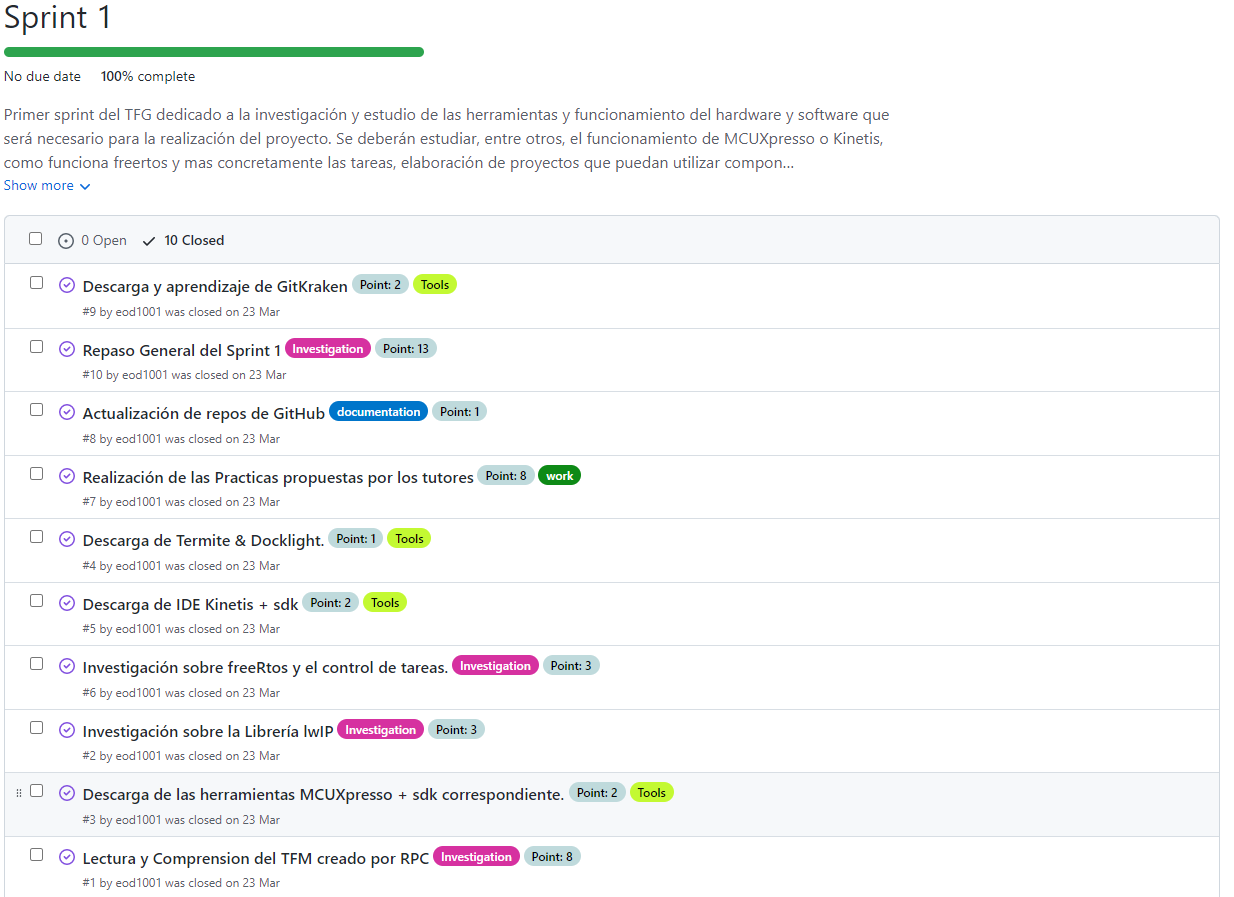
\includegraphics[width=0.9\textwidth]{Sprint1}
	\caption{Tareas planificadas para el Sprint1.}\label{sp1}
\end{figure}

Como podemos ver en la figura anterior, este primer Sprint se basó en la creación del entorno de trabajo y primeros pasos con las herramientas que iba a usar. Estos primeros pasos incluían ya la utilización de botones, leds y configuración de algún periférico.

\subsection{Sprint 2}
El sprint 2 recoge 9 tareas que suman 35 puntos de dificultad. Tuvo una duración de dos semanas y media. Este sprint estuvo enfocado a comenzar con la investigación del funcionamiento de lwIP. Cómo funcionaba y para qué servía, fueron los dos puntos más importantes. Tras entender estos dos puntos, busqué información sobre cómo implementarlo y comencé por la obtención de una IP según la mac de la placa y la creación de una tarea que pudiera recibir paquetes con información a través de este servicio. Para enviar los primeros paquetes utilicé Packet Sender.
\begin{itemize}
\item Investigación Protocolo TCP/IP y su implementación con lwIP.
\item Primeras partes del software.
\item Pruebas con la herramienta Packet Sender.
\end{itemize}

\imagen{Sprint2}{Tareas planificadas para el Sprint2.}


Otra parte a destacar fue el comienzo de la memoria con la herramienta Látex. Una herramienta que puede ser compleja de utilizar puesto que se debe aprender su sintaxis y acostumbrarse a un nuevo entorno para su uso.

\subsection{Sprint 3}
En este Sprint se buscó conseguir la comunicación de tres placas mediante el protocolo TCP/IP. En este punto, ya se disponía de conexión en red y de un \extranjerismo{`Listener'} que recibía paquetes de datos. El objetivo ahora era crear además, un \extranjerismo{`Writer'} capaz de enviarlos. Además, también se decidió la manera en que se transmitiría la información y sería en forma de comandos, por lo tanto también se implementó una especie de filtro que gestionaba el tipo de comando recibido en caso de existir. Por otro lado, también se comenzó a investigar e implementar las comunicaciones con los periféricos, concretamente con los motores y la pantalla. En este caso el sprint está constituido por 8 tareas que suman 36 puntos. Tareas principales:
\begin{itemize}
\item Creación del \extranjerismo{`Writer'}.
\item Creación del filtro de comandos.
\item Primeros pasos con UART y comunicación con los motores.
\item Primeros pasos con I2C y la pantalla LCD.
\end{itemize}

\imagen{Sprint3}{Tareas planificadas para el Sprint3.}

Este sprint tuvo una duración de dos semanas.

\subsection{Sprint 4}
En este Sprint se terminan, la comunicación de los motores y la de la pantalla, quedando operativas a falta de algunas mejoras. Además se produce uno de los hitos más importantes del proyecto, que es la investigación y abandono del procedimiento para la instalación del módulo wifi por falta de tiempo. En ese momento estaba comenzando las prácticas y se decide dejar apartada la parte de conexión inalámbrica para centrarme en la obtención de más funcionalidades. Esto viene dado porque desde la empresa en la que cursé las prácticas me ofrecieron la posibilidad de hacer algo que pudiera usarse en la fábrica.
Debido a esto, también me pongo a investigar sobre la posibilidad de introducir potenciómetros y sensores de temperatura para poder medir la temperatura de su CPD. El sprint suma una dificultad de 42 puntos en 8 tareas y se realizó en una semana y media. Tareas principales:
\begin{itemize}
\item Investigación sobre la implementación de un módulo WIFI, ESP8266.
\item Mejoras del código referente a la comunicación con los motores y la pantalla LCD.
\item Investigación e implementación de la lectura de los potenciómetros.
\end{itemize}

\imagen{Sprint4}{Tareas planificadas para el Sprint4.}

\subsection{Sprint 5}
Este sprint contiene 9 tareas llegando a un total de 32 puntos de dificultad. Es en este sprint donde se implementa la lectura del sensor de temperatura. Además se centran muchos esfuerzos en tratar de conseguir que todas las tareas funcionen adecuadamente. Se realizan multitud de pruebas y se trata de conseguir que la interacción con el usuario sea simple e intuitiva. Las tareas principales se resumen en:
\begin{itemize}
\item Mejora de usabilidad por el usuario.
\item Implementación del sensor de temperatura.
\item Mejora del código y funcionalidades de los periféricos.
\end{itemize}

\imagen{Sprint5}{Tareas planificadas para el Sprint5.}
La duración del sprint fue de una semana y media.
\subsection{Sprint 6}
Este Sprint se centra en dar los últimos retoques y completar la documentación a presentar para superar el TFG. Es el sprint más largo con 76 puntos de dificultad. En este caso se deberían haber separado en dos Sprints, pero puesto que todas las tareas se trataban sobre la documentación, se decidió dejar en solo uno. La duración de este sprint fue de dos semanas y media.
\begin{itemize}
\item Últimos retoques al código.
\item Generar la documentación de todo el trabajo.
\end{itemize}

\imagen{Sprint6}{Tareas planificadas para el Sprint6.}

\subsection{Diagrama de Gantt}
Para terminar con esta sección, se muestra el diagrama de Gantt seguido según la planificación temporal para la empresa, teniendo en cuenta festivos y fines de semana.

\begin{figure}[H]%
    \begin{center}%
    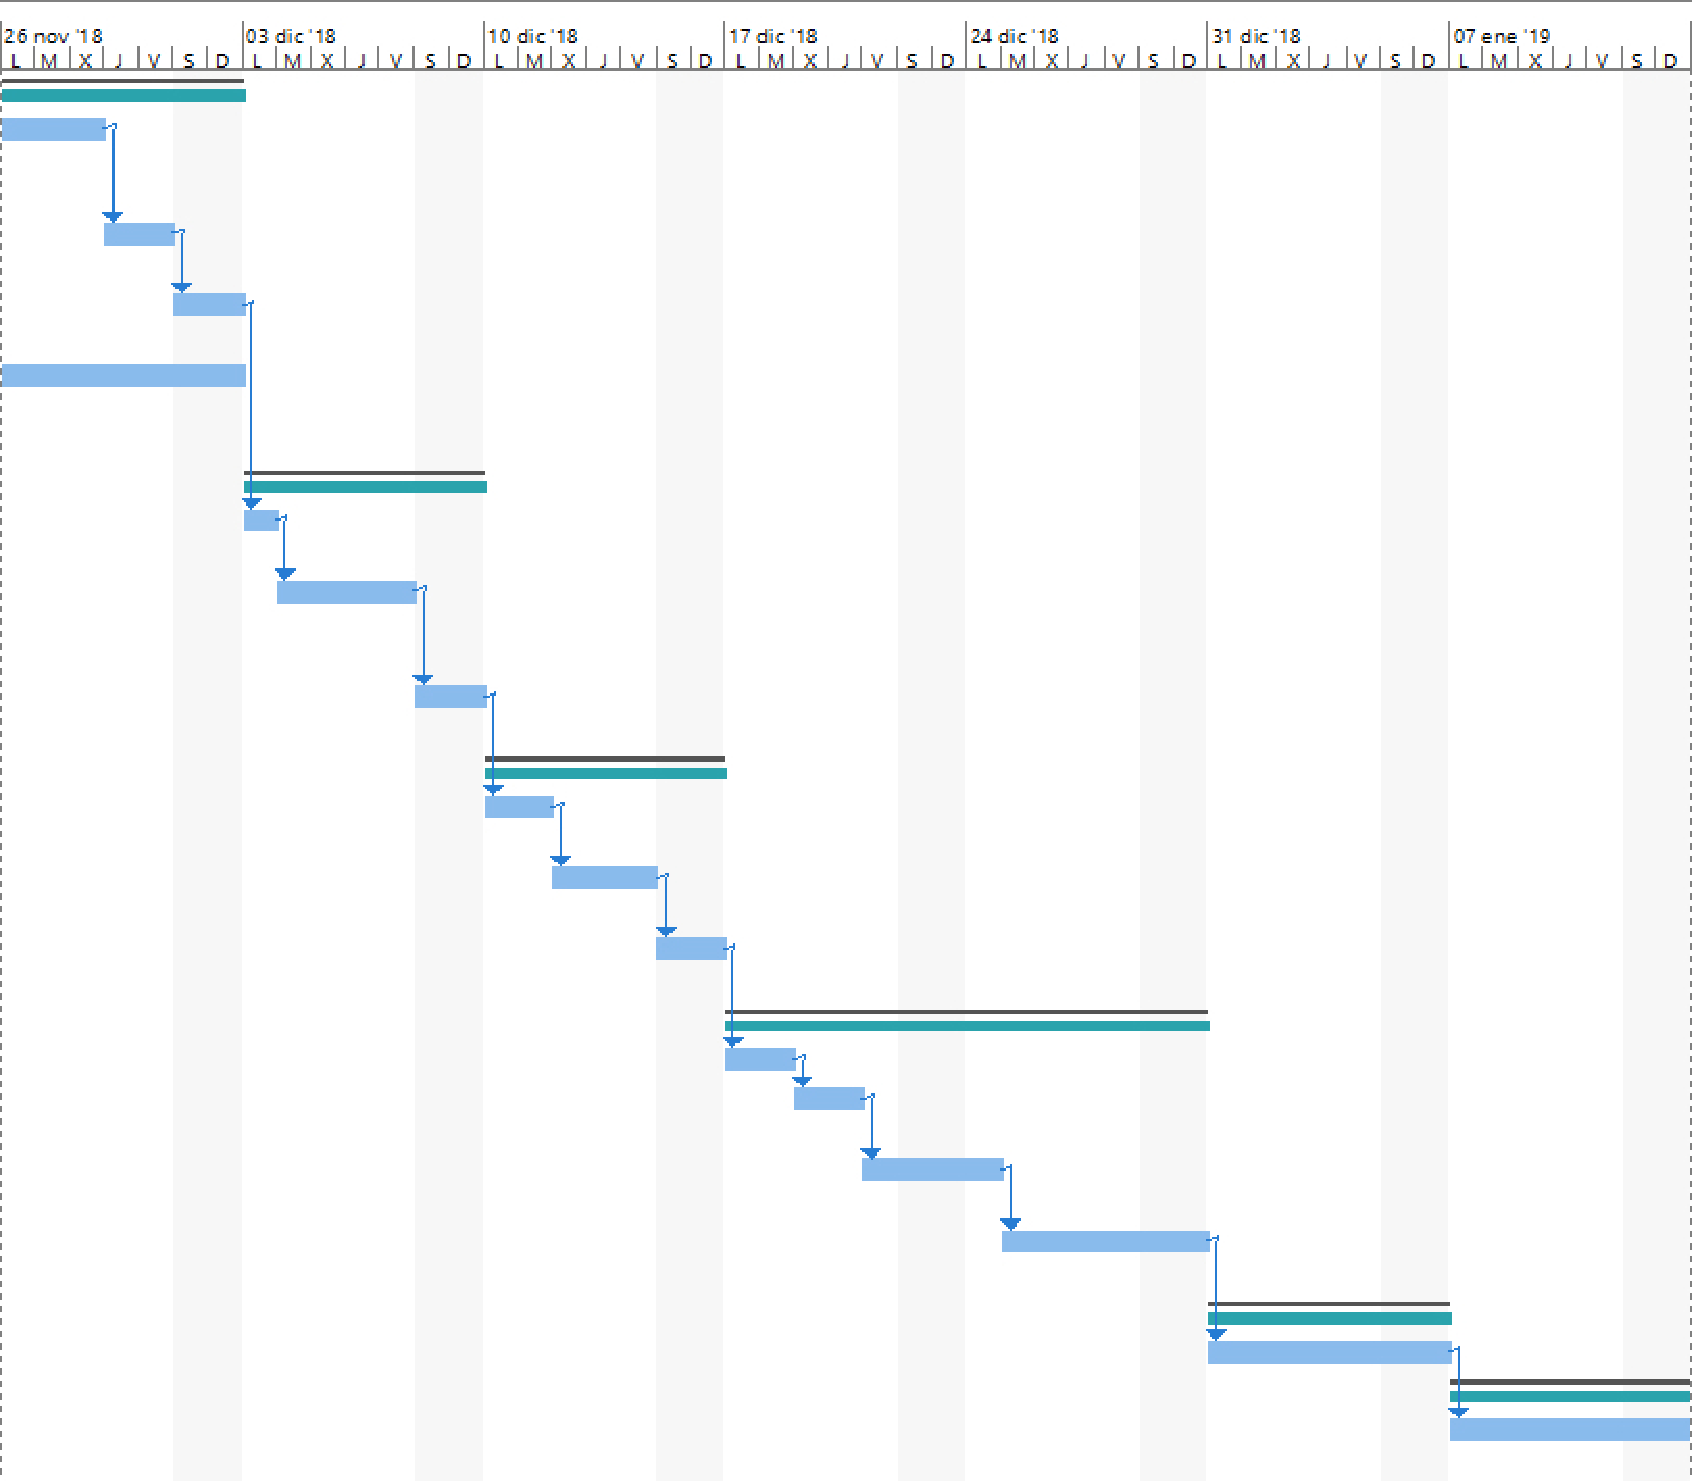
\includegraphics[angle=90,width=0.7\textwidth]{gantt1}%
    \caption{Diagrama de Gantt. Parte 1.}%
    \label{Dgantt1}%
    \end{center}%
  \end{figure}%
  
  \begin{figure}[H]%
    \begin{center}%
    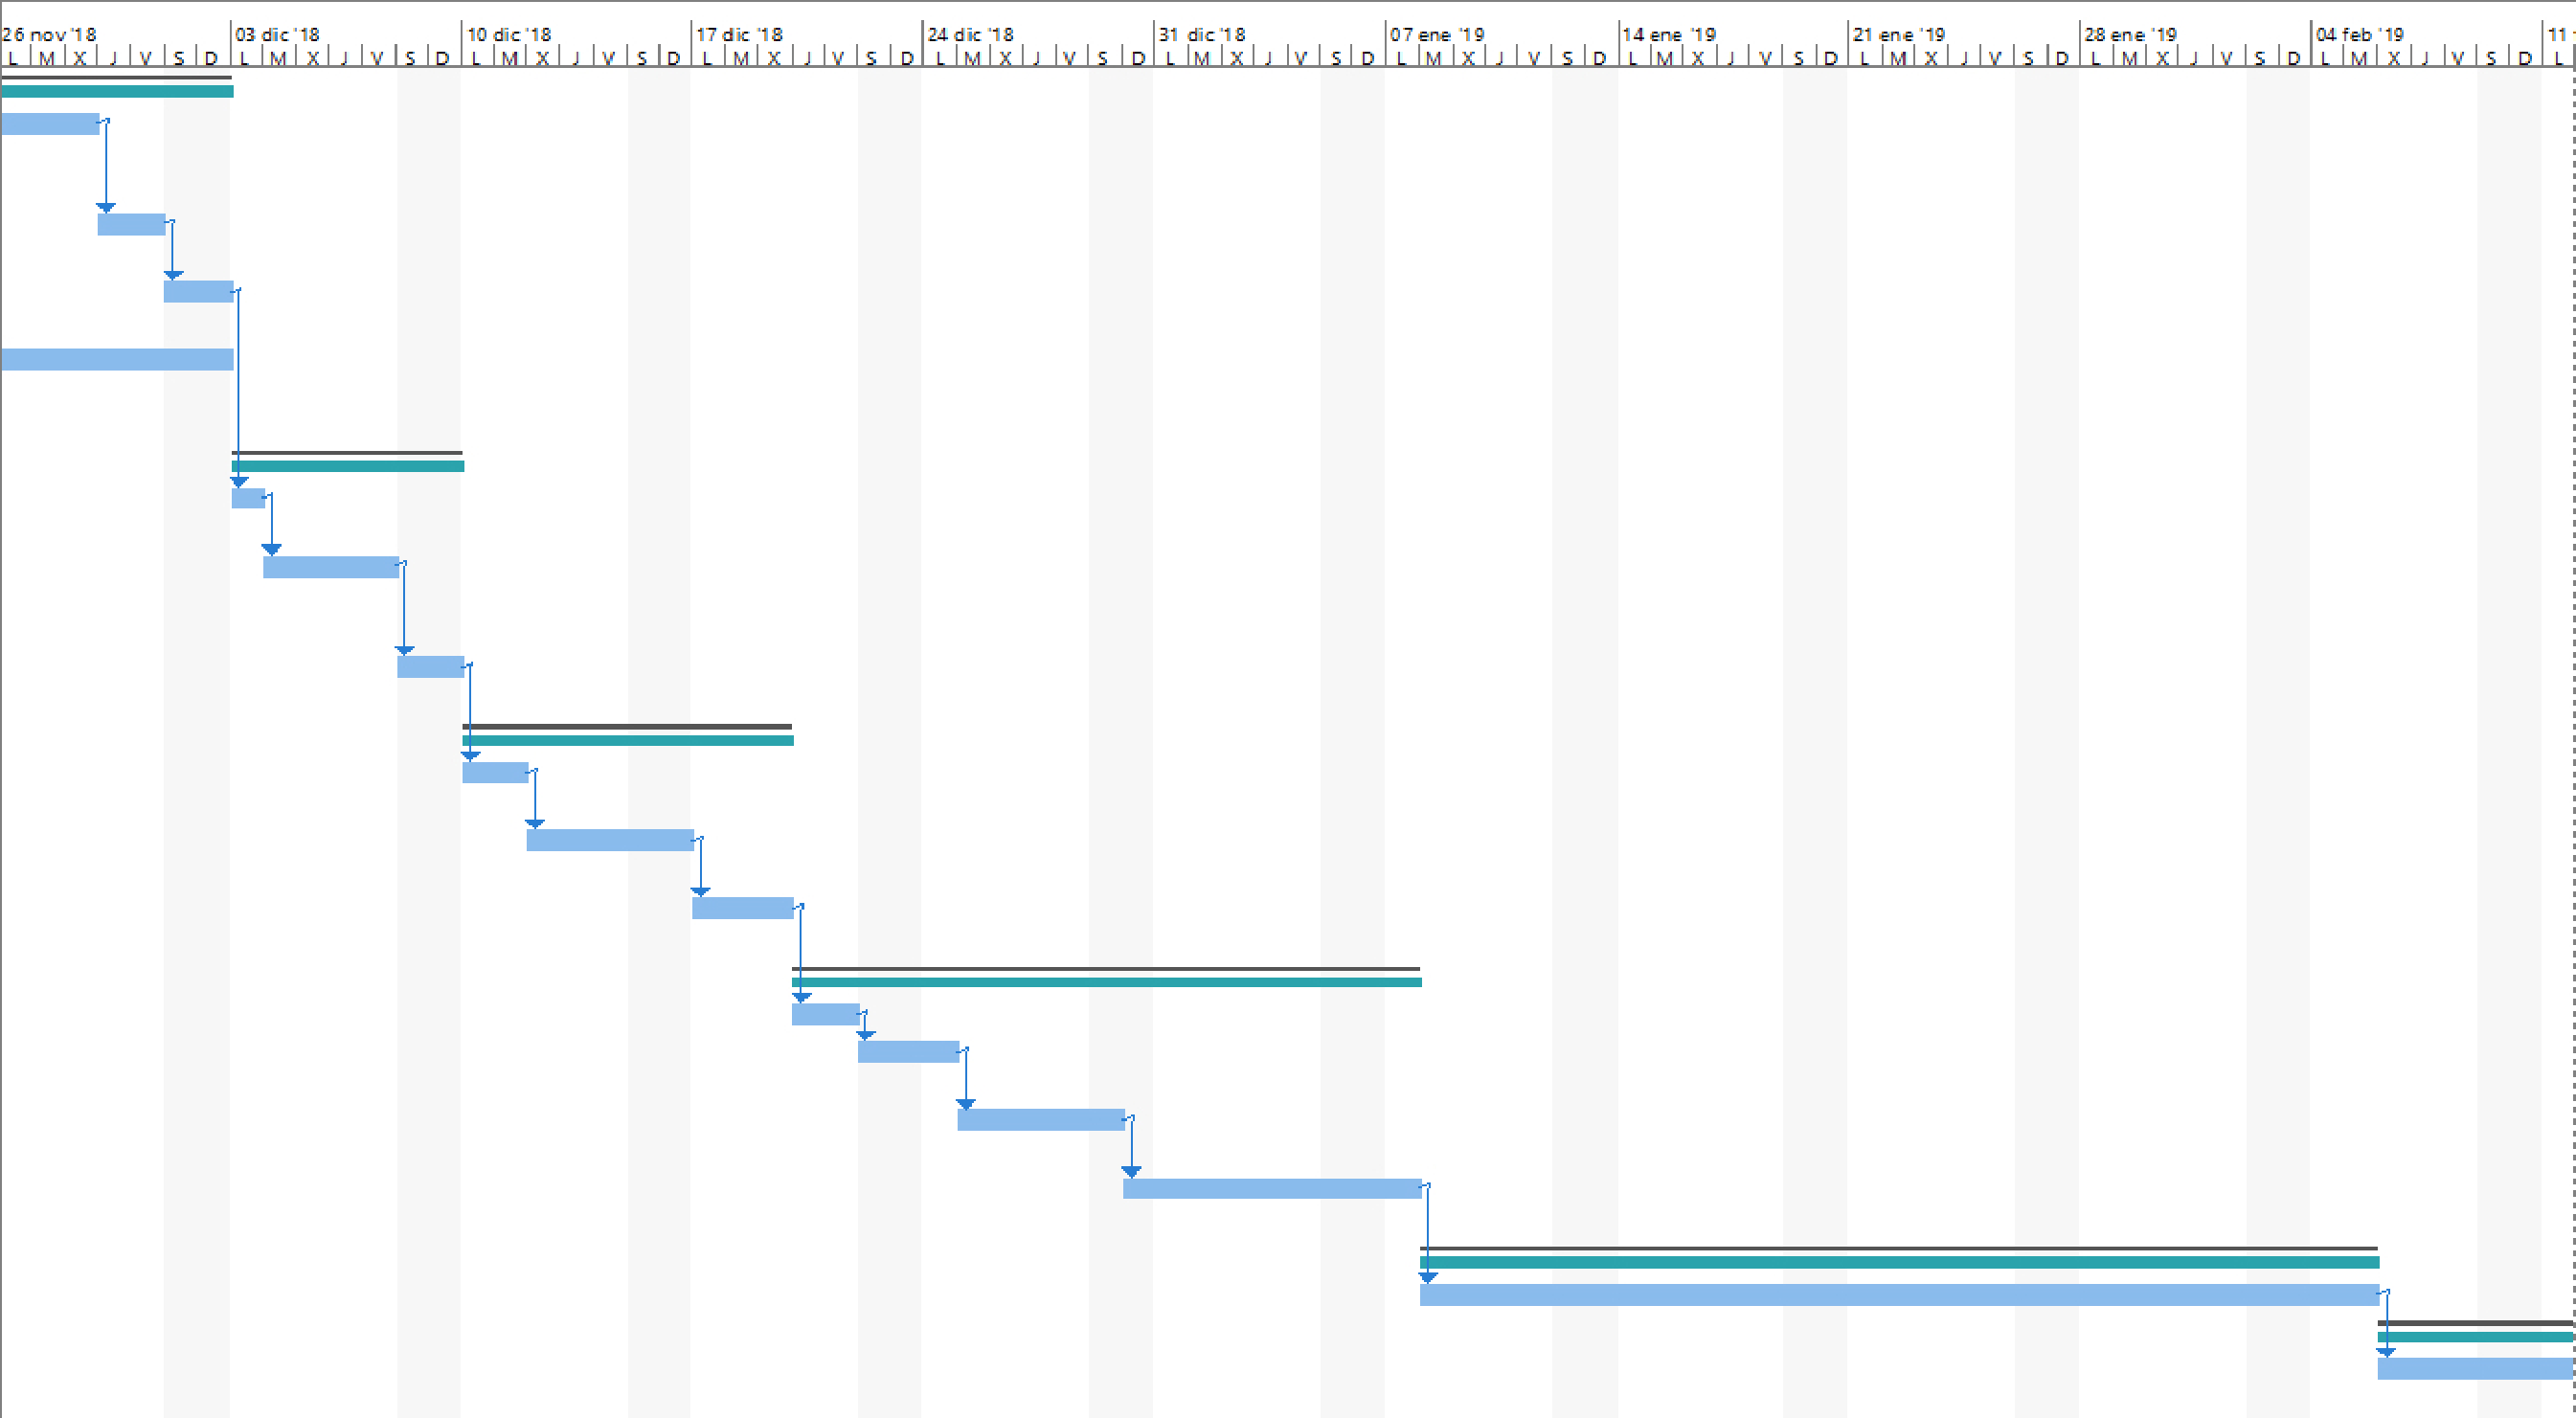
\includegraphics[angle=90,width=0.7\textwidth]{gantt2}%
    \caption{Diagrama de Gantt. Parte 2.}%
    \label{Dgantt2}%
    \end{center}%
  \end{figure}%

\section{Estudio de viabilidad}

\subsection{Viabilidad económica}
En este apartado se expone la viabilidad económica del desarrollo de este proyecto. Se tendrán en cuenta los gastos previstos durante el desarrollo y los beneficios, si los hubiera. Para calcularlo supondremos que el trabajo se hubiera desarrollado en el entorno real de una empresa. 

\subsubsection{Coste de personal.}
Para el desarrollo del producto final, vamos a suponer que se hubiera encargado una sola persona, durante un tiempo aproximado de 3 meses y 25 horas semanales. Supongamos que este trabajador junior tenga un salario bruto de 1500 euros al mes. 
Para conocer el salario neto lo haremos con la siguiente formula \cite{calculadoraSantander}:
\begin{equation} \label{eq:salario}
  salario\ bruto - IRPF - SS = salario\ neto
\end{equation}
Por lo que el trabajador recibiría el siguiente salario:
\begin{equation} \label{eq:salario}
  1500\text{\euro} - 10,49\% - 6,35\% = 1247,4\text{\euro}
\end{equation}
Para la realización de la fórmula anterior se han utilizado los tramos mas altos de la autonomía de Castilla y León \cite{escalaCyL} y la escala a nivel nacional que podemos encontrar en \cite{agenciaTributaria}. El cálculo está simplificado al no tener en cuenta la progresividad de la escala de tramos.


\subsubsection{Costes pertenecientes a la SS.}
Sobre el salario bruto, se producen retenciones y pagos a la Seguridad Social. De estos impuestos algunos los paga la empresa y otros el trabajador. En este apartado se van a calcular los importes de estas retenciones, para ello, tomaremos como referencia la tabla de bases de cotización de la Seguridad Social. En esta tabla, deberemos buscar el grupo que nos corresponda, en este caso ``Ingenieros y Licenciados. Personal de alta dirección no incluido en el artículo 1.3. c) del Estatuto de los Trabajadores''. Este grupo tiene unas bases mínimas de 1466,40€/mes. Y unas máximas de 4070,10€/mes.

\tablaSmallSinColores{Costes pertenecientes a la SS}{l l l}{costes-ss}
{\multicolumn{1}{l}{Concepto} & Empresa & Trabajador\\}
{
  Contingencias comunes & 23,60\% & 4,70\%\\
  Desempleo             &  5,50\% & 1,55\%\\
  FOGASA                &  0,20\% & 0,00\%\\
  Formación             &  0,60\% & 0,10\%\\
  \textbf{Total}        & \textbf{29,9\%} & \textbf{6,35\%}\\
}

Como podemos observar en la figura anterior los costes que la empresa debe asumir son el 29,9\% del salario del trabajador y el trabajador sufriría una retención del 6,35\% 

\subsubsection{Coste total de personal}
Para hallar el coste total del desarrollo del proyecto calcularemos la siguiente formula.
\begin{equation} \label{eq:salario}
  (salario\ mensual + costes\ ss) \times n^{o}\ meses = coste\ total
\end{equation}

De modo que el coste total se obtiene así:
\begin{equation} 
  (1500\text{\euro} + 448,5\text{\euro}) * 3 = 5845,5\text{\euro}
\end{equation}

La siguiente tabla recoge diferentes costes asociados al personal y 
su coste total.

\tablaSmallSinColores{Coste total de personal}{l l}{personal}
{\multicolumn{1}{l}{Concepto} & Coste\\}
{
  Salarios          & \EUR{1800}\\
  Seguridad Social  & \EUR{448,5}\\
  Meses             & 3 meses\\
  \textbf{Total}    & \textbf{\EUR{5845,5}}\\
}


\subsubsection{Costes del hardware.}
Como ya vimos en la memoria para el desarrollo de este proyecto, se han necesitado varios dispositivos. Aquí surge un inconveniente puesto que, según se recoge en la ley de impuestos sobre sociedades \cite{BasesyTiposSS} se necesitan 8 años para amortizar los equipos relacionados con la rama de la información, pero la renovación de este tipo de hardware se debe realizar en un periodo mucho menor, de 4 años. En este caso he optado por realizar los cálculos con un periodo de 4 años. Quedaría de la siguiente manera:

El coste mensual de un dispositivo se calcula así:
\begin{equation} \label{eq:coste-hw}
  Coste\ del\ dispositivo\ /\ Periodo\ de\ amortización\ (en\ meses)
\end{equation}

Por lo tanto, el coste de un dispositivo es el siguiente:
\begin{equation} \label{eq:coste-amor-hw}
  Coste\ mensual\ amortizado\ \times n^{o}\ meses\
\end{equation}

Para desarrollar cómodamente este software se ha utilizado una estación de trabajo portátil de 1000€ y un monitor de 24 pulgadas que tiene un coste de aproximadamente 150€.
\tablaSmallSinColores{Coste del \extranjerismo{hardware}}{l l l}{coste-hw}
{\multicolumn{1}{l}{\extranjerismo{Hardware}} & Coste & Coste amortizado\\}
{
  Entorno de trabajo & \EUR{1150} & \EUR{71,87}\\
  \textbf{Total}      & \EUR{1150} & \textbf{\EUR{71,87}}\\
}


\subsubsection{Costes del software.}

Para el desarrollo del proyecto, se han utilizado varios programas y aplicaciones. Según la ley del impuesto sobre sociedades \cite{ImpSoc}, el máximo de años para realizar la amortización de sistemas y programas informáticos es de 6 años. Sin embargo, al igual que hicimos en el apartado de los costes hardware, se calculará en un periodo de 4 años.
Es importante tener en cuenta que la mayoría de programas utilizados se encuentran bajo licencias que permiten su uso sin coste, por lo que no aparecerán en la tabla de costes de software.
Por otro lado, gran parte del software utilizado se usa mediante suscripción, por lo que su coste aparecerá computado bajo su suscripción determinada.

\tablaSmallSinColores{Coste del \extranjerismo{software}}{l l l}{coste-sw}
{\multicolumn{1}{l}
{\extranjerismo{Software}}              & Coste        & Coste amortizado\\}
{
  Windows 10 Pro\cite{win10pro} & \EUR{259}    & \EUR{21,58}\\
  Office 365\cite{office365}    & \EUR{126}    & \EUR{31,5}\\
  \textbf{Total}                        & \EUR{385} & \textbf{\EUR{53,08}}\\
}


\subsubsection{Coste del sistema empotrado.}
Veamos los costes de los componentes utilizados para el laboratorio.

\tablaSmallSinColores{Coste del Sistema Empotrado}{c c c c}{coste-SE}
{\multicolumn{1}{l}{\extranjerismo{Hardware}} & Coste & Unidades & Coste Total\\}
{
  Placas FRDM-K64F\cite{CosteK64f}    & \EUR{42,36} & 3 & \EUR{127,08}\\
  Shield Arduino\cite{costeShield}  & \EUR{21,50} & 1 & \EUR{21,50}\\
  Pantalla LCD\cite{CosteLcd}         & \EUR{14,58} & 1 & \EUR{14,58}\\
  Motores\cite{CosteMotores}          & \EUR{70,57} & 2 & \EUR{141,14}\\
  Placa Motores\cite{CostePlacaMotor} & \EUR{93,46} & 1 & \EUR{93,46}\\
  Switch\cite{CosteSwitch}            & \EUR{10,95} & 1 & \EUR{10,95}\\
  Cables de Red\cite{CosteEthernet}   & \EUR{2,55} & 3 & \EUR{7,65}\\
  Cables \cite{CosteCables}           & \EUR{5,12} & 1 & \EUR{5,12}\\
  \textbf{Total}                      & - & - & \textbf{\EUR{421,48}}\\
}


\subsubsection{Coste total del proyecto}
A continuación se muestra el coste total asignado a todo el proyecto:

\tablaSmallSinColores{Coste total del proyecto}{l l}{coste-total}
{\multicolumn{1}{l}
{Tipo de coste}            & Coste        \\}
{ 
  Personal                 & \EUR{5845,5} \\
  \extranjerismo{Hardware} & \EUR{71,87} \\
  \extranjerismo{Software} & \EUR{53,08} \\
  Componentes del SE       & \EUR{421,48}  \\
  \textbf{Total}           & \textbf{\EUR{6391.93}} \\
}

\subsubsection{Beneficios del proyecto}
Es importante mencionar que el SE no tiene una función comercial específica y por lo tanto no se tiene un beneficio económico. El proyecto se ha realizado como investigación para que en el futuro se puedan crear sistemas de SE semejantes, rentabilizando los costes producidos por este proyecto. Por lo tanto, no se consideran los gastos como pérdidas sino como una inversión generada con el objetivo de la adquisición de competencias.


\subsection{Viabilidad legal}
En cuanto a la viabilidad legal, encontramos que la parte más importante sería el conocimiento y utilización de licencias. Las licencias establecen una serie de términos y condiciones en los que se pueden utilizar los softwares de terceros. En el próximo apartado, veremos cuales son las licencias que se han usado durante el desarrollo de este proyecto.

\subsubsection{Licencias utilizadas en el desarrollo del SE}
En esta subsección, se muestran las licencias que tiene el software de terceros que se ha utilizado para la creación del programa presentado:
\begin{itemize}
\item ``The 3-Clause BSD License'' (BSD-3): Bajo este tipo de licencia estaría el software generado por MCUXpresso y lwIP. Esta licencia permite crear y distribuir nuevo software a partir de los programas que estén adscritos a este tipo de licencia.
\item Apache 2.0: Hay una parte del código del procesador de la placa que pertenece a ARM Limited y se encuentra bajo la licencia de Apache 2.0. Esta licencia permite el uso, copia, modificación y redistribución del código.
\item El código perteneciente a FreeRTOS es propiedad de Amazon.com, Inc. Se permite el uso, copia, modificación, publicación, distribución, volver a licenciar y comercializar, manteniendo siempre el aviso de derechos de autor.
\end{itemize}


\subparagraph{Licencias para el SE}

Puesto que se pretende que el software realizado sea abierto, se publicará bajo la licencia Apache 2.0 \cite{infoApache}. Podemos ver sus características en la \ref{tabla:apache}.


\tablaSmallSinColores{Licencia Apache 2.0}{l l l l}{apache}
{\multicolumn{1}{l}
{Permisos}        & Condiciones                & Limitaciones    \\}
{ 
  Uso comercial   & Aviso de licencia          & Uso de marcas registradas \\
  Modificación    & y derechos de autor        & Responsabilidad           \\
  Distribución    & Declaración de los cambios & Garantía                  \\ 
  Uso en patentes \\
  Uso privado     \\
}
\subparagraph{Utilización de la licencia Apache}
Para indicar a terceros que el software realizado se encuentra bajo la licencia Apache, se expone en el directorio raíz un fichero que recibe el nombre de `License' con el siguiente texto:

\begin{quotation}
  Copyright [yyyy] [name of copyright owner] \bigskip

  Licensed under the Apache License, Version 2.0 (the "License");
  you may not use this file except in compliance with the License.
  You may obtain a copy of the License at \bigskip
  
  \quad http://www.apache.org/licenses/LICENSE-2.0 \bigskip

  Unless required by applicable law or agreed to in writing, software
  distributed under the License is distributed on an ``AS IS'' BASIS,
  WITHOUT WARRANTIES OR CONDITIONS OF ANY KIND, either express or implied.
  See the License for the specific language governing permissions and
  limitations under the License.
\end{quotation}

Por supuesto se deberáN modificar los apartados que se encuentran entre corchetes e introducir el año y nombre del propietario del software. La inclusión de este texto en un trabajo, permite que quede constancia de que se le aplica la licencia de Apache 2.0 \cite{LicenciaApache}

\subsubsection{Licencia para la documentación}

En el caso de la licencia de la documentacion, escogemos una licencia diferente y mas adecuada como es el caso de Creative Commons Atribución-NoComercial-CompartirIgual 4.0 Internacional
(CC BY-NC-SA 4.0) \cite{creativeCommons}.

La licencia permite:
\begin{itemize}
\item Que la obra realizada pueda ser compartida libremente
\item Que pueda ser copiada y redistribuida.
\item Que se pueda editar y crear nuevos ficheros partiendo de la original.
\end{itemize}
Como obligación para todo aquel que utilice este proyecto se requiere exponer la autoría del autor del trabajo original  y sea presentada bajo la misma licencia que posee la original.


\tablaSmallSinColores{Licencia CC BY-NC-SA 4.0}{l l l l}{ccbyncsa4}
{\multicolumn{1}{l}
{Permisos}      & Condiciones                & Limitaciones    \\}
{ 
  Distribución  & Crédito al autor           & Responsabilidad           \\  
  Modificación  & Aviso de licencia          & Uso de patentes           \\
  Uso privado   & y derechos de autor        & Uso de marcas registradas \\
                & Declaración de los cambios & Garantía                  \\ 
                & No comercial               &                           \\ 
                & Mismo licenciamiento       &                           \\ 
}

El uso de la licencia queda expuesto mediante el logo de Creative Commons y un pequeño texto que lo acompaña, indicando a los lectores de la obra que está protegida bajo los derechos y obligaciones de esa licencia.


\apendice{Especificación de requisitos} \label{Ap:requisitos}

\section{Introducción}

En este apéndice se exponen los requisitos del software creado y la funcionalidad de este. Para ello, se da un descripción completa de las funciones que debe realizar el programa y de cómo un usuario podría utilizarlo. Se definen los pasos y opciones para utilizar correctamente el hardware del sistema empotrado y que cumpla así con su función. Por otro lado, se definen también los requisitos no funcionales. Para la exposición de estos requisitos se seguirán algunos estándares como el IEEE 830\-1998 \cite{IEEE8301998} o el IEEE 29148\-2011 \cite{IEEE291482011}.

\subsection{Audiencia destinataria}
Este documento tiene como destinatario, cualquier persona que quiera iniciarse en el ámbito de los sistemas embebidos. Tanto alumnos, como profesores u otros usuarios interesados, podrán encontrar información sobre comunicaciones con periféricos y entre SE, y para qué y cómo pueden utilizarse. 

Para la exposición de las siguientes secciones se utilizarán, por motivo de simplicidad, algunas abreviaciones:
\begin{description}
\item[Sistema empotrado o embebido.] SE
\item[Software del sistema empotrado.] SW del SE
\item[Requisito de interfaces externas.] RE
\item[Requisito funcional.] RF
\item[Requisito no funcional.] RNF
\item[Casos de Uso.] CU
\end{description}

\subsection{Objetivos generales}
En esta sección vamos a ver los objetivos para el funcionamiento del SE:
\begin{itemize}
\item Configurar un SE para que pueda conectarse en red mediante cable y comunicarse utilizando TCP/IP 
\item Gestionar el hardware de la planta piloto mediante envío de comandos software entre placas
\end{itemize}
A partir de estos dos objetivos principales vamos a continuar viendo en los demás apartados los requisitos que tiene la planta piloto.

\subsection{Tipos de usuario}
Para la utilización del sistema empotrado no se necesita ningún tipo de conocimiento técnico por lo que cualquier persona interesada puede usarlo sin problemas. La mayor dificultad radica en conectar los componentes correctamente, conocer los casos de uso del SE y los pasos para utilizar la placa `maestro'. 
Teniendo en cuenta que junto con el software se proporcionan varios documentos:
\begin{itemize}
\item Manual del usuario.
\item Manual del programador.
\item Casos de uso de la planta piloto.
\end{itemize} 
Cualquier usuario podría utilizarlo atendiendo a esos documentos.

\section{Catálogo de requisitos}
\subsection{Requisitos externos}
\begin{itemize}
  	
	\item \textbf{RE-1 Acceso a la red.} El SE tiene que ser capaz de usar Ethernet para conectarse en red. RE de alta prioridad.
	\item \textbf{RE-2 Transmisiones en red.} El SE tiene que ser capaz de usar el protocolo TCP/IP para comunicarse con otros sistemas embebidos. RE de alta prioridad.
	\item \textbf{RE-3 Uso de Botones.} Los seis botones disponibles en la placa más el shield deben poderse utilizar correctamente.  RE de media prioridad.
	\item \textbf{RE-4 Uso de dispositivos ADC.} Tanto el sensor de temperatura como los potenciómetros deben realizar adecuadamente sus lecturas. RE de alta prioridad.
	\item \textbf{RE-5 Uso de pantalla LCD} La pantalla debe mostrar los mensajes requeridos correctamente. RE de media prioridad
	
\end{itemize}

\subsection{Requisitos Funcionales}
\begin{itemize}
  	\item \textbf{RF-1 Recepción de comandos} El SE tiene que recibir comandos transmitidos mediante paquetes TCP con destino a su correspondiente dirección IP y puerto TCP abierto. RF de alta prioridad.
  	\item \textbf{RF-2 Identificación de comandos} El SE tiene que ser capaz de identificar los comandos recibidos para poder ejecutar las acciones correctas. RF de alta prioridad
  	\item \textbf{RF-3 Movimiento de los motores} Los motores deben realizar correctamente su giro dependiendo del comando recibido. RF de alta prioridad.
  	\item \textbf{RF-4 Obtención de la velocidad de los motores} La obtención de los valores de velocidad de los motores debe ser recibida sin demora y correctamente. RF de media prioridad.
  	\item \textbf{RF-5 Obtención de la temperatura} La obtención de los valores de temperatura debe ser recibida sin demora y correctamente. RF de media prioridad.
  	\item \textbf{RF-6 Envío de comandos} Los comandos se deben enviar por red y no deben perderse en el proceso de comunicación. RF de alta prioridad.
  	\item \textbf{RF-7 Parada de ambos motores} La parada de ambos motores al pulsar el `botón de emergencia' debe ser rápida y completa. RF de alta prioridad.
  	\item \textbf{RF-8 Comunicación I2C} La comunicación con la pantalla LCD debe ser mediante I2C. RF de alta prioridad.
	\item \textbf{RF-9 comunicación UART} La comunicación con los motores mediante UART debe ser rápida y confiable. RF de alta prioridad.
\end{itemize}

\subsection{Requisitos No Funcionales}
\begin{itemize}
  	\item \textbf{RNF-1 Hardware del SE} El SE tiene que ser desarrollado con una placa de desarrollo FRDM-K64F. RNF de alta prioridad.
  	\item \textbf{RNF-2 Rendimiento del SE} El SE tiene que ser capaz de realizar las acciones indicadas por el usuario sin demora. RNF de media prioridad.
  	\item \textbf{RNF-3 Seguridad del SE} El SE tiene que asegurar que sus componentes no presentan riesgos eléctricos al usuario. RNF de alta prioridad. 
  	\item \textbf{RNF-4 Calidad del SW} El SW tiene que garantizar cierto nivel de calidad, tales como incluir comentarios que faciliten su comprensión para un mantenimiento o portabilidad posteriores. RNF de media prioridad.
  	\item \textbf{RNF-5 Usabilidad del SE} La utilización del sistema debe ser sencilla para el usuario. RNF de alta prioridad.
  	\item \textbf{RNF-6 Conectividad física de los componentes} Los elementos que componen el sistema deben estar conectados de manera adecuada. RNF de alta prioridad.
\end{itemize}



\section{Especificación de requisitos}

\subsection{Diagrama de Casos de Uso}

En la figura \ref{casosDeUso} se muestran los casos de uso que un usuario puede llevar a cabo con la planta piloto.

%\imagen{casosUso}{Diagrama de casos de uso.} \label{casosDeUso}
\begin{figure}[H]%
    \begin{center}%
    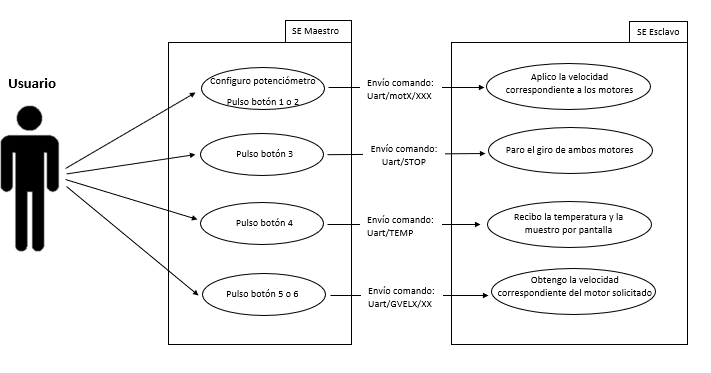
\includegraphics[angle=90,width=0.6\textwidth]{casosUso}%
    \caption{Diagrama de casos de uso.}%
    \label{casosDeUso}%
    \end{center}%
  \end{figure}%

\subsection{Casos de Uso}
Las siguientes tablas muestran los requisitos de los casos de uso:

\tablaSmallSinColores{CU-1 Set Speed A.}{l l}{cu-1}
{\multicolumn{1}{l}
{CU-1}                          & Set Speed A \\}
{ 
  \textbf{Versión}              & 1.0     \\
  \textbf{Fecha}                & 2022-06 \\
  \textbf{Requisitos asociados} & RF-3   \\
  \textbf{Descripción}          & Fijar la velocidad del Motor A\\ 
  \textbf{Precondición}         & \parbox{.5\textwidth}{\begin{itemize}
  	\item Se debe tener conexión en red entre las placas.
    \item Todos los elementos del sistema deben estar conectados
    \end{itemize}}\\
  \textbf{Acciones}             & \parbox{.5\textwidth}{\begin{enumerate}
    \item El usuario ajusta el potenciómetro 1 según sus necesidades.                         
    \item El usuario pulsa el botón 1 para enviar el comando.
    \item Se corrobora mediante la pantalla LCD y los leds de la placa maestro que se ha enviado el comando.
  \end{enumerate}}\\
  \textbf{Postcondición}        & El motor comienza a moverse\\
  \textbf{Excepciones}          & \parbox{.5\textwidth}{\begin{itemize}
    \item Si alguno de los elementos del sistema no está bien conectado o no se dispone de corriente no funcionará  
    \item La lectura del potenciómetro puede no realizarse bien en algunas ocasiones.
  \end{itemize}}\\
  \textbf{Importancia}          & Alta    \\
  \textbf{Comentarios}          & \parbox{.5\textwidth}{\begin{itemize}
  	\item Los cuatro leds de la placa shield se irán encendiendo a medida que avance el envío del comando
  	\end{itemize}}\\
}


\tablaSmallSinColores{CU-2 Set Speed B.}{l l}{cu-2}
{\multicolumn{1}{l}
{CU-2}                          & Set Speed B \\}
{ 
  \textbf{Versión}              & 1.0     \\
  \textbf{Fecha}                & 2022-06 \\
  \textbf{Requisitos asociados} & RF-3   \\
  \textbf{Descripción}          & Fijar la velocidad del Motor B\\ 
  \textbf{Precondición}         & \parbox{.5\textwidth}{\begin{itemize}
  	\item Se debe tener conexión en red entre las placas
    \item Todos los elementos del sistema deben estar conectados
    \end{itemize}}\\
  \textbf{Acciones}             & \parbox{.5\textwidth}{\begin{enumerate}
    \item El usuario ajusta el potenciómetro 2 según sus necesidades.                         
    \item El usuario pulsa el botón 2 para enviar el comando.
    \item Se corrobora mediante la pantalla LCD y los leds de la placa maestro que se ha enviado el comando.
  \end{enumerate}}\\
  \textbf{Postcondición}        & El motor comienza a moverse\\
  \textbf{Excepciones}          & \parbox{.5\textwidth}{\begin{itemize}
    \item Si alguno de los elementos del sistema no está bien conectado o no se dispone de corriente no funcionará  
    \item La lectura del potenciómetro puede no realizarse bien en algunas ocasiones.
  \end{itemize}}\\
  \textbf{Importancia}          & Alta    \\
  \textbf{Comentarios}          & \parbox{.5\textwidth}{\begin{itemize}
  	\item Los cuatro leds de la placa shield se irán encendiendo a medida que avance el envío del comando
  	\end{itemize}}\\
}



\tablaSmallSinColores{CU-3 Parada de Emergencia.}{l l}{cu-3}
{\multicolumn{1}{l}
{CU-3}                          & Parada de emergencia \\}
{ 
  \textbf{Versión}              & 1.0     \\
  \textbf{Fecha}                & 2022-06 \\
  \textbf{Requisitos asociados} & RF-7   \\
  \textbf{Descripción}          & Parada de emergencia de ambos motores\\ 
  \textbf{Precondición}         & \parbox{.5\textwidth}{\begin{itemize}
    \item Se debe tener conexión en red entre las placas
    \item Todos los elementos del sistema deben estar conectados
    \end{itemize}}\\
  \textbf{Acciones}             & \parbox{.5\textwidth}{\begin{enumerate}
    \item El usuario pulsa el botón 3 para enviar el comando.
    \item Se corrobora mediante la pantalla LCD y los leds de la placa maestro que se ha enviado el comando.
  \end{enumerate}}\\
  \textbf{Postcondición}        & Ambos motores se paran\\
  \textbf{Excepciones}          & \parbox{.5\textwidth}{\begin{itemize}
    \item Si alguno de los elementos del sistema no está bien conectado o no se dispone de corriente no funcionará  
    \item La lectura del potenciómetro puede no realizarse bien en algunas ocasiones.
  \end{itemize}}\\
  \textbf{Importancia}          & Alta    \\
  \textbf{Comentarios}          & \parbox{.5\textwidth}{\begin{itemize}
    \item Los cuatro leds de la placa shield se encenderán a la vez.
    \end{itemize}}\\

} 

\tablaSmallSinColores{CU-4 Obtener Temperatura.}{l l}{cu-4}
{\multicolumn{1}{l}
{CU-4}                          & Obtener temperatura \\}
{ 
  \textbf{Versión}              & 1.0     \\
  \textbf{Fecha}                & 2022-06 \\
  \textbf{Requisitos asociados} & RF-5    \\
  \textbf{Descripción}          & El usuario solicita la temperatura ambiente.\\    
     \textbf{Precondición}      & \parbox{.5\textwidth}{\begin{itemize}
    \item Se debe tener conexión en red entre las placas.
    \item Todos los elementos del sistema deben estar conectados.
    \end{itemize}}\\
  \textbf{Acciones}             & \parbox{.5\textwidth}{\begin{enumerate}
    \item El usuario pulsa el botón 4.
      \item Se corrobora mediante la pantalla LCD y los leds de la placa maestro que se ha enviado el comando.

  \end{enumerate}}\\
  \textbf{Postcondición}        & \parbox{.5\textwidth}{\begin{itemize}
  	\item La temperatura se muestra en la pantalla de la placa esclavo 1.
  	\end{itemize}}\\
  \textbf{Excepciones}          & \parbox{.5\textwidth}{\begin{itemize}
    \item Si alguno de los elementos del sistema no está bien conectado o no se dispone de corriente no funcionará  
  \item Las dos primeras lectura del sensor de temperatura son de calibración.
  \end{itemize}}\\
  \textbf{Importancia}          & Alta    \\
     \textbf{Comentarios}       & Los leds de la placa shield se encenderán a la vez\\}
     

\tablaSmallSinColores{CU-5 Obtener Velocidad Motor A.}{l l}{cu-5}
{\multicolumn{1}{l}
{CU-5}                          & Obtener Velocidad Motor A \\}
{ 
  \textbf{Versión}              & 1.0     \\
  \textbf{Fecha}                & 2022-06 \\
  \textbf{Requisitos asociados} & RF-4   \\
  \textbf{Descripción}          & Obtener velocidad del Motor A\\ 
  \textbf{Precondición}         & \parbox{.5\textwidth}{\begin{itemize}
    \item Se debe tener conexión en red entre las placas.
    \item Todos los elementos del sistema deben estar conectados
    \end{itemize}}\\
  \textbf{Acciones}             & \parbox{.5\textwidth}{\begin{enumerate} 
    \item El usuario pulsa el botón 5 para enviar el comando.
    \item Se corrobora mediante la pantalla LCD y los leds de la placa maestro que se ha enviado el comando.
  \end{enumerate}}\\
  \textbf{Postcondición}        & \parbox{.5\textwidth}{\begin{itemize}
	\item Se muestra por la pantalla LCD la velocidad del motor A.
  	\end{itemize}}\\
  \textbf{Excepciones}          & \parbox{.5\textwidth}{\begin{itemize}
    \item Si alguno de los elementos del sistema no está bien conectado o no se dispone de corriente no funcionará  
  \end{itemize}}\\
  \textbf{Importancia}          & Alta    \\
  \textbf{Comentarios}          & \parbox{.5\textwidth}{\begin{itemize}
    \item Los cuatro leds de la placa shield se encenderán al mismo tiempo
    \end{itemize}}\\
    }
  
  
  
\tablaSmallSinColores{CU-6 Obtener Velocidad Motor B.}{l l}{cu-6}
{\multicolumn{1}{l}
{CU-6}                          & Seleccionar SE \\}
{ 
  \textbf{Versión}              & 1.0     \\
  \textbf{Fecha}                & 2022-06 \\
  \textbf{Requisitos asociados} & RF-4   \\
  \textbf{Descripción}          & Obtener velocidad del Motor B\\ 
  \textbf{Precondición}         & \parbox{.5\textwidth}{\begin{itemize}
    \item  Se debe tener conexión en red entre las placas.
    \item Todos los elementos del sistema deben estar conectados.
    \end{itemize}}\\
  \textbf{Acciones}             & \parbox{.5\textwidth}{\begin{enumerate} 
    \item El usuario pulsa el botón 6 para enviar el comando.
    \item Se corrobora mediante la pantalla LCD y los leds de la placa maestro que se ha enviado el comando.
  \end{enumerate}}\\
  \textbf{Postcondición}        & \parbox{.5\textwidth}{\begin{itemize}
  	\item Se muestra por la pantalla LCD la velocidad del motor B.
  	\end{itemize}}\\
  \textbf{Excepciones}          & \parbox{.5\textwidth}{\begin{itemize}
    \item Si alguno de los elementos del sistema no está bien conectado o no se dispone de corriente no funcionará.
  \end{itemize}}\\
  \textbf{Importancia}          & Alta    \\
  \textbf{Comentarios}          & \parbox{.5\textwidth}{\begin{itemize}
    \item Los cuatro leds de la placa shield se encenderán al mismo tiempo.
    \end{itemize}}\\
    
}




\apendice{Especificación de diseño} \label{ch:design}

\section{Introducción} \label{sec:design-intro}
Tras recoger las especificaciones de los requisitos del \sw{} se 
puede comenzar con la especificación del diseño. Este apéndice detalla
las soluciones tomadas respecto al diseño del \sw{}.

Con el diseño del \sw{} se trata de dar respuesta a cuestiones relativas a los
datos, y su representación; las división lógica en módulos, y su funcionamiento
interno; y como estructurar el \sw{} arquitectónicamente.

\subsection{Ámbito del \sw{}} \label{sec:design-ambito}
El \sw{} a desarrollar debe permitir a un usuario operar con un
sistema empotrado de forma remota a través de una aplicación web. Al ser
entidades tan diferenciadas, tanto el sistema empotrado como la aplicación web
tienen que contar con \sw{} propio y específico a cada plataforma.

El \sw{} del sistema empotrado tiene que residir en el propio sistema. Con su
ejecución se pretende actuar sobre el \hw{} habilitado a tal fin.

En cuanto al \sw{} de la aplicación web, ejecutado en un servidor de aplicaciones, va a
servir como interfaz de usuario frente al sistema empotrado que le va a permitir
ordenar la ejecución de las funciones del sistema empotrado.



\section{Diseño de datos} \label{sec:design-datos}
Para que la aplicación web pueda ordenar al sistema empotrado actuar de una
determinada manera se precisa de la transmisión de unos comandos concretos. En
consecuencia, se tiene que definir la estructura de los comandos para que ambos
\extranjerismo{softwares} sean capaces de entenderse.


\subsection{Transferencia de los comandos} \label{sec:design-transferencia}
Los comandos van a ser transferidos usando el protocolo Transmission Control
Protocol (TCP). El protocolo está orientado a la conexión y se encarga de
establecerla la comunicación mediante unos mensajes de sincronización (SYN) y
reconocimiento (ACK), como se puede ver en \ref{fig:tcp}.

\begin{figure}[!h]
  \centering
  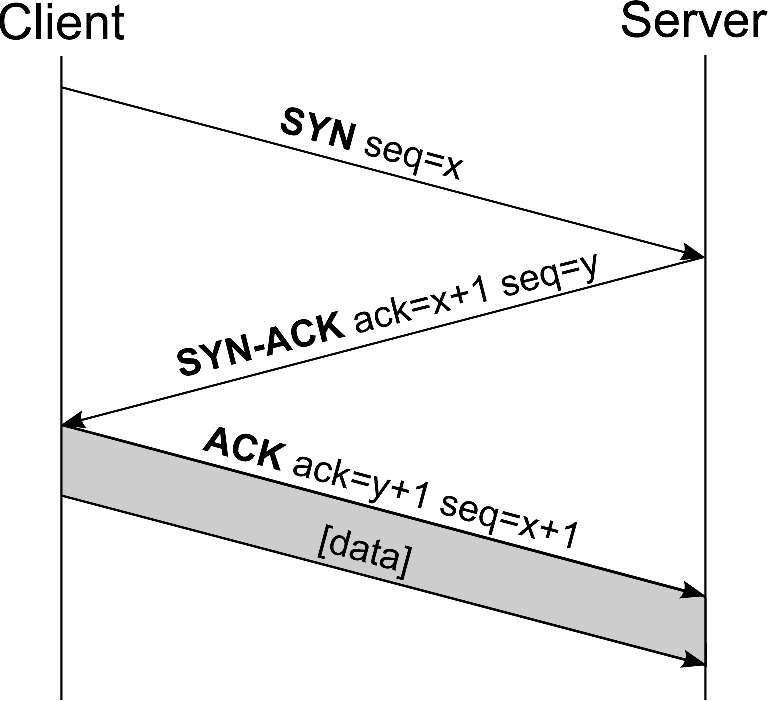
\includegraphics[width=0.6\textwidth]{tcp}
  \caption{Conexión TCP \cite{webpage:tcp-handshake}} \label{fig:tcp}
\end{figure}

Aprovechando que el protocolo TCP se encarga establecer una conexión fiable,
se delega en él el establecimiento de la conexión y los comandos serán enviados
después encapsulados dentro de segmentos TCP.


\subsection{Comando LED} \label{sec:design-datos-led}
Con este comando se indica al sistema empotrado que muestre una luz con el color
indicado. Hay un LED para cada uno de los tres colores primarios: rojo, verde y
azul. Aunque los LED pueden encenderse individualmente, encendiéndolos
simultáneamente se pueden combinar los colores primarios y generar otros
nuevos. Los colores obtenidos por adición son el cian, magenta, amarillo y
blanco. Además, debe ser posible que los LED se apaguen y dejen de iluminar.

Para conseguir lo anterior, el nombre del comando refleja la alusión a los LED
RGB. El comando se acompaña de un argumento que especifica el color concreto a
iluminar. Para ayudar a diferenciar el comando del argumento se ubica un carácter
separador.

\tablaSmallSinColores{Comando LED}{l c c c c}{comando-led}
{\multicolumn{1}{l}{Color} & Comando & Separador & Argumento & Comando resultante\\}
{
  Rojo     & led & : & r & led:r \\
  Verde    & led & : & g & led:g \\
  Azul     & led & : & b & led:b \\
  Cian     & led & : & c & led:c \\
  Magenta  & led & : & m & led:m \\
  Amarillo & led & : & y & led:y \\
  Blanco   & led & : & w & led:w \\
  No color & led & : & o & led:o \\
}


\subsection{Comando MSG} \label{sec:design-datos-msg}
Este comando indica al sistema empotrado que muestre una cadena de caracteres
en la pantalla LCD. Como la pantalla tiene dos líneas, se necesita indicar
la línea donde mostrar el texto.

El nombre del comando refleja que trata con los mensajes de texto. El comando
se acompaña de un argumento que especifica la línea donde escribir la cadena de
caracteres. Después se añade otro argumento con la cadena de caracteres a
mostrar. Como en el resto de comandos, entre el comando y cada uno de los
argumentos se ubica un carácter separador. 

\tablaSmallSinColores{Comando MSG}{l c c c c c c}{comando-msg}
{\multicolumn{1}{l}{Línea} & Comando & S. & Arg. 1 & S.
                           & Arg. 2 & Comando resultante\\}
{
  1\textsuperscript{a} línea & msg & : & 0 & : & <chars> & msg:0:<chars>\\
  2\textsuperscript{a} línea & msg & : & 1 & : & <chars> & msg:1:<chars>\\
}


\subsection{Comando PWM} \label{sec:design-datos-pwm}
Este comando indica al sistema empotrado que regule la intensidad del brillo de
los LED compatibles con PWM. El sistema empotrado cuenta con 4 LED regulables
por lo que es necesario identificar cual de ellos hay que regular.

El nombre del comando refleja que se van a utilizar los LED PWM. Como hay 4 LED
hace falta un argumento que permita seleccionar el LED a regular. Para indicar
la intensidad se añade otro argumento con el valor nuevo, entre 0 y 100.
De nuevo, entre el comando y cada uno de los argumentos se ubica un carácter
separador. Por último, se añade de nuevo un carácter con el color de LED para
indicar al sistema empotrado que ha finalizado el valor numérico. 

\tablaSmallSinColores{Comando PWM}{l c c c c c c c}{comando-pwm}
{\multicolumn{1}{l}{LED} & Comando & S. & Arg. 1 & S.
                           & Arg. 2 & Fin & Cmd. resultante\\}
{
  Blanco   & pwm & : & w & : & <0-100> & w & pwm:w:<0-100>w \\
  Verde    & pwm & : & g & : & <0-100> & g & pwm:g:<0-100>g \\
  Amarillo & pwm & : & y & : & <0-100> & a & pwm:y:<0-100>a \\
  Rojo     & pwm & : & r & : & <0-100> & r & pwm:r:<0-100>r \\
}



\section{Diseño arquitectónico} \label{sec:arch}
La arquitectura de un \sw{} se describe en el estándar IEEE 42010-2011
\cite{webpage:ieee42010-2011} como  los ``conceptos fundamentales o propiedades
de un sistema en su entorno encarnados por sus elementos, relaciones, y en los
principios de su diseño y evolución.''

Así pues, como los entornos del \sw{} del sistema empotrado y de la aplicación
web están tan diferenciados, se opta por usar estilos arquitectónicos diferentes
y adaptados a cada \sw{}.

\subsection{Diseño arquitectónico del SE} \label{sec:arch-se}
Los sistemas empotrados se relacionan con el entorno en el que se encuentran
mediante actuadores y sensores, y dependiendo de su finalidad, con
restricciones de tiempo real. La organización del \sw{} debe ajustarse a estas
realidades.

En sistemas sistemas simples sin restricciones de tiempo se puede organizar
el \sw{} de forma simple. En cambio, cuando las tareas de un sistema empotrado
tienen que responder rápidamente a eventos con restricciones de tiempo se hace
necesario organizar el \sw{} de forma más compleja.

En un sistema empotrado sin restricciones se podría utilizar la arquitectura
del \sw{} más simple conocida como Round Robin. Las tareas del sistema empotrado
se ejecutan dentro de un bucle principal, en ellas se examina el estado \hw{} y
de ser necesario se realiza el tratamiento correspondiente. Una vez terminada
una tarea, se ejecuta la siguiente, y al completar la última se vuelve a empezar
el ciclo con la primera de todas.

\imagenalto{arch_rr}{Tareas en bucle infinito}{!h}{0.5}

Para no tener que estar sondeando constantemente el \hw{}, se puede mejorar la 
arquitectura anterior incluyendo interrupciones. Estas señales permiten indicar
al sistema empotrado cuando ha ocurrido un evento y lo libera del sondeo
constante.

Si bien ambas arquitecturas serían factibles de aplicar al sistema empotrado,
con intención de dar respuesta al requisito no funcional sobre el rendimiento
y respuesta del sistema se va a usar una arquitectura basada en un Sistema
operativo en tiempo real (RTOS).

La decisión se fundamenta en la flexibilidad y el tiempo de respuesta que el
RTOS es capaz de proporcionar. Cada función del sistema se implementa dentro de
una tarea individual con una determinada prioridad. El RTOS se encarga de 
planificar el orden de ejecución de las tareas en base a la prioridad de cada
de ellas. 

Por lo tanto, una tarea con prioridad alta, porque necesita un tiempo
de respuesta estricto, es ejecutada antes que las demás. Más aún, se puede
configurar el RTOS para que desaloje una tarea de menor prioridad y pase a
ejecutar una de mayor prioridad.

\begin{figure}[!h]
  \centering
  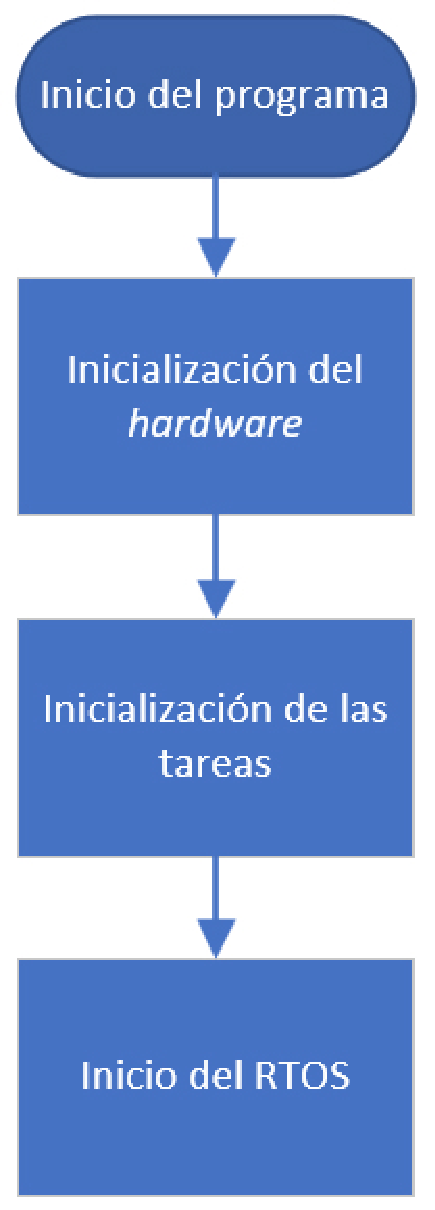
\includegraphics[height=0.5\textheight]{arch_bucle}
  \caption{Bucle principal del \sw{}} \label{fig:bucle}
\end{figure}

\begin{figure}[!h]
  \centering
  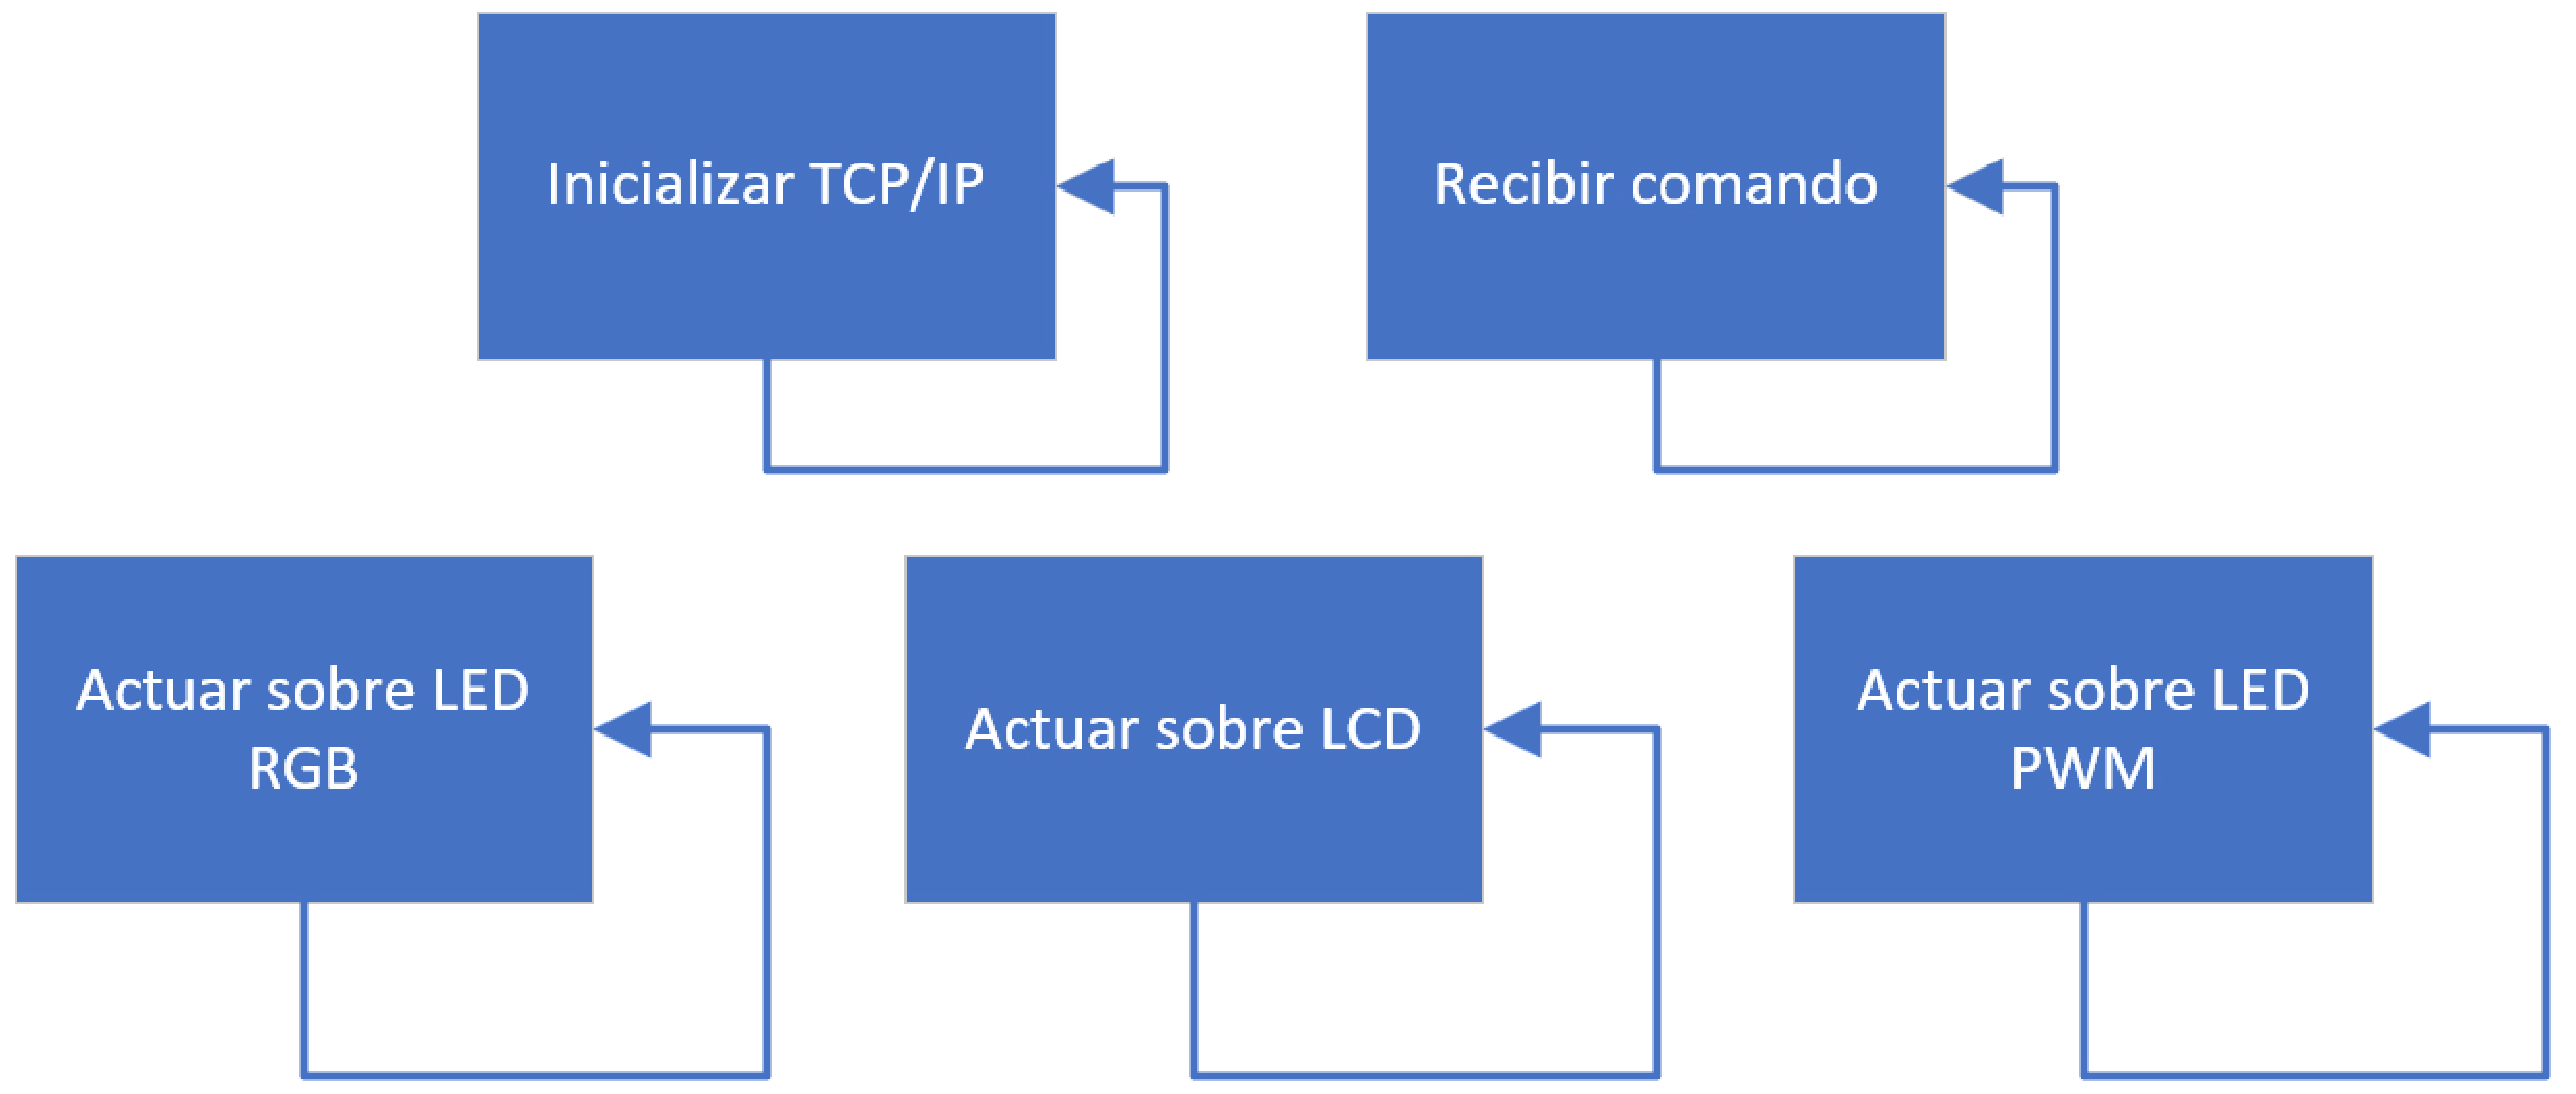
\includegraphics[width=0.6\textheight]{arch_tareas}
  \caption{Tareas para el RTOS} \label{fig:tareas}
\end{figure}

Con las tareas \ref{fig:tareas} se da respuesta a los casos de usos planteados
para el sistema empotrado durante la especificación de los requisitos del \sw{}.
Gracias la flexibilidad que aporta esta solución se podrían añadir o remover
funciones rápidamente. Por ejemplo, bastaría con agregarlas o quitarlas del 
RTOS durante la inicialización \ref{fig:bucle}.


\subsection{Diseño arquitectónico de la aplicación web} \label{sec:arch-aw}
Por lo que se refiere al \sw{} de aplicación web, representa un cambio de
contexto completo. La aplicación se encuentra alojada en un servidor de
aplicaciones que permite al usuario acceder a la interfaz web desde un
navegador web cualquiera.

La tecnología a utilizar en conjunción con el servidor de aplicaciones es
JavaServer Faces (JSF) \cite{webpage:jsf}. Su especificación concreta su
propósito para construir aplicaciones web e interfaces de usuarios basadas
en componentes. Cada componente de \sw{} sirve para encapsular un conjunto
de funciones o datos estrechamente relacionados.

Además, JSF utiliza el patrón de arquitectura Modelo-Vista-Controlador (MVC).
Este patrón separa la lógica de la aplicación en tres componentes diferenciados.
Con la separación se impulsa el desarrollo modular, facilitando la colaboración
y la reutilización durante el desarrollo.

Los tres componentes de MVC son:
\begin{description}
  \item[Modelo:] Define los datos y su estructura empleados por la aplicación.
  Si los datos se modifican, la vista se actualiza para reflejar los cambios.
  \item[Vista:] Define la interfaz y como se muestran los datos al usuario
  en ella.
  \item[Controlador:] Contiene la lógica responsable de manipular el modelo
  en función de las acciones del usuario.
\end{description}

\imagenancho{arch_mvc}{Relación entre MVC y el usuario}{!h}{0.8}

\subsubsection{Diseño del modelo} \label{sec:arch-modelo}
En JSF el modelo se define mediante \extranjerismo{beans}. Los
\extranjerismo{beans} se crean con clases Java. Están compuestos por una
conjunto de atributos y sus correspondientes métodos 
\extranjerismo{getters} y \extranjerismo{setters}.

Así pues, el valor de un atributo, también llamado propiedad, se consulta con
su correspondiente método \extranjerismo{get} y se puede actualizar con su
método \extranjerismo{set}.

\subsubsection{Diseño de la vista} \label{sec:arch-vista}
En JSF la vista se define mediante ficheros escritos en Extensible HyperText
Markup Language (XHTML) que incluyen etiquetas especiales para añadir
componentes específicos de JSF. Posteriormente, el código de los ficheros XHTML
es traducido a código Hypertext Markup Language (HTML) interpretable por los
navegadores web.

La conexión entre la interfaz y el resto de la aplicación se realiza con ayuda
del Lenguaje de Expresiones de JSF (EL). Con estas expresiones se enlazan los
componentes de la interfaz con las propiedades de los \extranjerismo{beans}.

\subsubsection{Diseño del controlador} \label{sec:arch-ctl}
En JSF el controlador se puede definir con \extranjerismo{beans} al igual
que en el modelo \ref{sec:arch-modelo}. Pero a diferencia de los
\extranjerismo{beans} del modelo, los \extranjerismo{beans} del controlador
cuentan con los métodos necesarios para realizar la lógica de negocio
requerida por la aplicación.


\subsection{Diseño conjunto del sistema} \label{sec:design-comp}

\imagenancho{componentes}{Diagrama de componentes del sistema}{!h}{1}


\subsection{Diagramas de clases} \label{sec:design-comp}

\imagenancho{pkg-controller}{Diagrama de clases de los paquetes
\extranjerismo{controller} y \extranjerismo{controller.network}}{H}{0.9}

\imagenalto{pkg-model}{Diagrama de clases del paquete
\extranjerismo{model}}{H}{0.3}


\subsection{Diseño de la interfaz} \label{sec:design-iface}
Para que el usuario pueda controlar el sistema empotrado, la aplicación web
pone su disposición una interfaz web. En una sola página el usuario puede
ver las funciones disponibles y operar con ellas.

En primer lugar la interfaz tiene que permitir que el usuario introduzca
los datos de conexión con el sistema empotrado.

\imagenancho{panel_datos}{Introducción de datos}{!h}{0.9}

Una vez establecidos los datos se muestran unos paneles con las funciones
disponibles.

Con unos botones se puede escoger el color iluminado por los LED RGB.

\imagenancho{panel_led}{Panel para cambiar el color de los LED RGB}{!h}{0.9}

En unos cuadros de texto, el usuario puede introducir un mensaje y pulsando
un botón lo puede enviar.
\imagenancho{panel_msg}{Panel para enviar un texto al LCD}{!h}{0.9}

\clearpage

Con unos controles deslizantes, el usuario puede cambiar la intensidad del brillo
de los LED regulados por PWM.
\imagenancho{panel_pwm}{Panel para regular el brillo de los LED PWM}{!h}{0.9}

\clearpage

La interfaz completa se construye según lo definido en el siguiente diseño.

\begin{figure}[H]
  \centering
  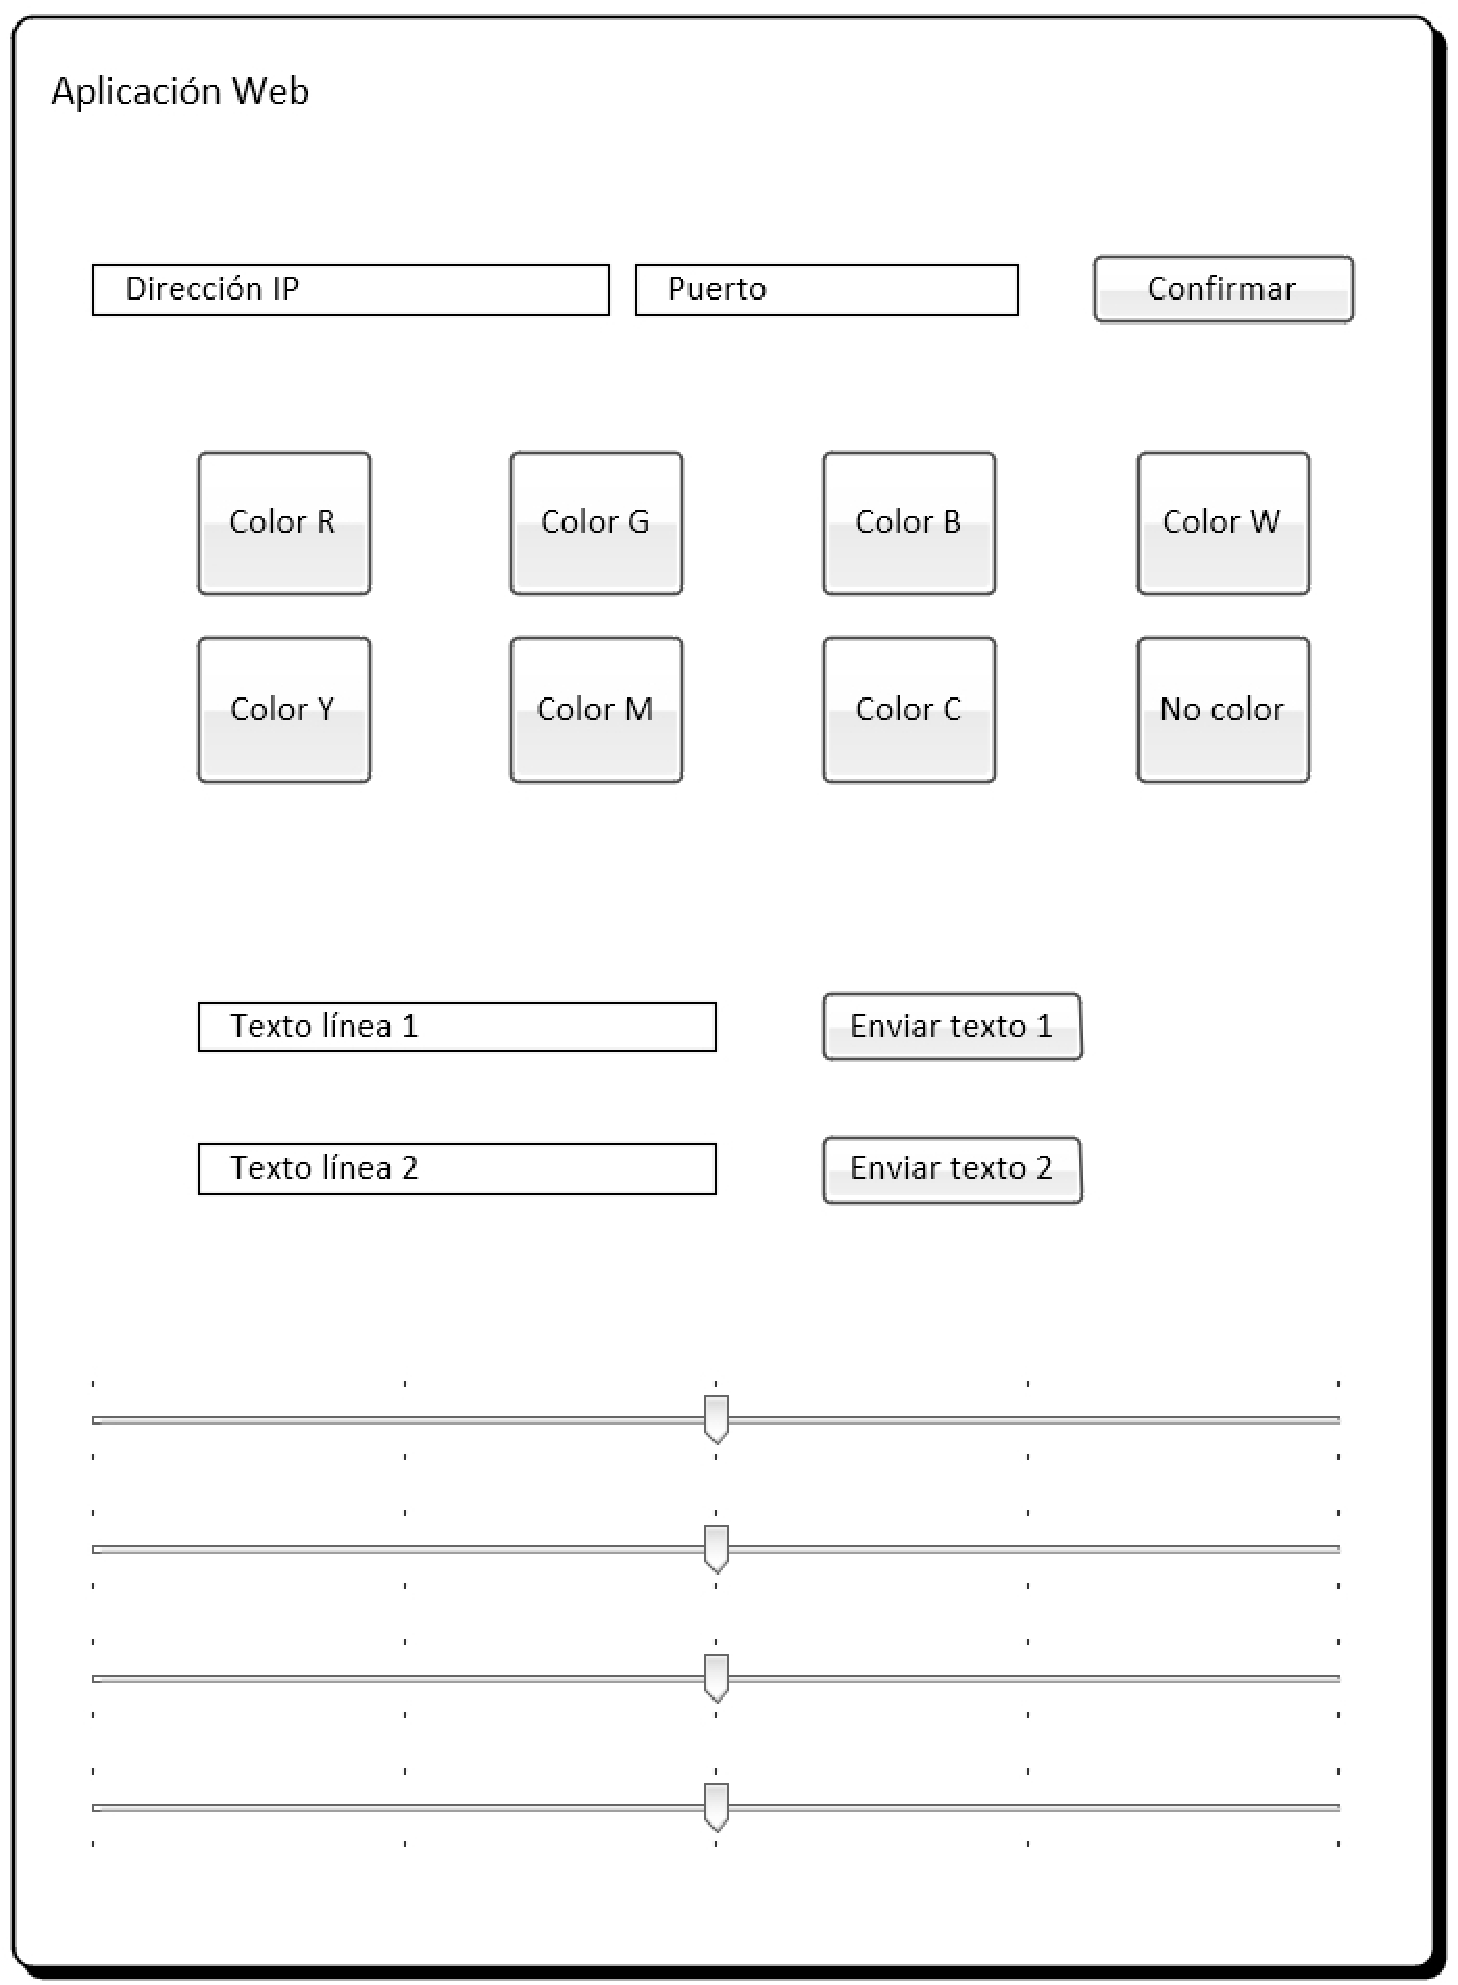
\includegraphics[width=0.55\textheight]{interfaz}
  \caption{Diseño de la interfaz} \label{fig:intefaz}
\end{figure}

\clearpage

\section{Diseño procedimental} \label{sec:design-proc}
El siguiente diagrama muestra las interacciones que se producen entre
los componentes del sistema desde que el usuario solicita una función hasta que
el sistema empotrado la realiza.

\figuraApaisadaSinMarco{0.9}{secuencia}{Diagrama de secuencia}{fig:secuencia}{}

\apendice{Documentación técnica de programación}

\section{Introducción}
Este apéndice muestra las herramientas necesarias para entender y poder reutilizar el software presentado. Sin embargo, no es necesario utilizar las mismas herramientas, pero es muy recomendable.
Para el desarrollo del trabajo se ha utilizado MCUXpresso. A continuación se muestra cómo instalar y configurar este IDE. Además, también veremos otras herramientas que nos ayudarán a comprobar el correcto funcionamiento del software.

\section{Estructura de directorios}
Antes de comenzar la instalación de MCUXpresso veamos de que ficheros disponemos en este proyecto.
La estructura de directorios es:

\begin{figure}[!h]
	\centering
	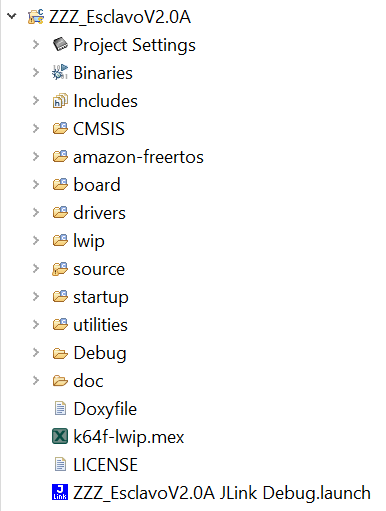
\includegraphics[width=0.5\textwidth]{directorios}
	\caption{Estructura de directorios.}
\end{figure}
\FloatBarrier

\begin{description}
  \item[/] Directorio raíz, contiene el resto de los directorios. Se incluyen ficheros como LICENSE que contiene los términos y condiciones del licenciamiento del software y el fichero .MEX que contiene los datos de las configuraciones de los pines, relojes y periféricos. Este último fichero lo genera el propio IDE. En la raíz también encontramos los archivos binarios para la ejecución del programa y el archivo para realizar el debug.
  \item[/CMSIS/] Cortex Microcontroller Software Interface Standard (CMSIS). Reúne las fuentes que proporcionan interfaces al procesador y sus periféricos.
  \item[/amazon-freertos/] Fuentes relacionadas con FreeRTOS, sistema operativo en tiempo real usado en el proyecto.
  \item[/board/] Fuentes autogenerados por el IDE que permiten habilitar y configurar el hardware de la placa de desarrollo.
  \item[/doc/] Documentación del proyecto.
  \item[/drivers/] Controladores necesarios para trabajar con el hardware.
  \item[/lwip/] Fuentes relativos a lwIP, la implementación de la pila de protocolos TCP/IP.
  \item[/source/] Código fuente del proyecto. El fichero main.c es el que contiene el código del funcionamiento de las placas. Además se encuentran los ficheros que agrupan herramientas para completar la ejecución de las funciones utilizadas en el main.c.
  \item[/startup/] Código de arranque generado por el IDE.
  \item[/utilities/] Código generado por el IDE con utilidades auxiliares usadas para depuración o registro de eventos.
\end{description}

\section{Manual del programador}
\subsection{Descarga e instalación de MCUXpresso}
En primer lugar será necesario descargar el IDE desde la página oficial de NXP. Este software estará en la pestaña de desarrolladores. Para poder descargarlo será necesario tener una cuenta de NXP, la cual es gratuita y te puedes registrar fácilmente desde el sitio web.
Dicho esto, iniciamos sesión en la página vamos a la pestaña en la que se encuentra el software y pinchamos en descargar \cite{DLMCUX}. 

\imagen{DIDLE}{Pagina de descarga del IDE.}

Una vez hecho esto, elegimos el sistema operativo donde se ejecutará nuestro IDE. El instalador sigue los pasos habituales en este tipo de instalaciones, aceptar la licencia, elegir la ubicación donde se guardarán los archivos y controladores de programa, etc. Podemos dejar todas estas opciones por defecto o variarlas a nuestro gusto. 
Al descargar el IDE viene con él la herramienta Config Tools que nos ayudará a realizar la configuración a bajo nivel de la placa. 



Una vez tenemos instalado MCUXpresso, lo abrimos. Lo primero que nos pide es elegir una ruta donde guardar nuestros proyectos. Es recomendable que sea una ruta fácilmente accesible pues nos será de gran ayuda poder llegar rápidamente y poder importar y exportar de manera más sencilla los proyectos que necesitemos.

\begin{figure}[!h]
	\centering
	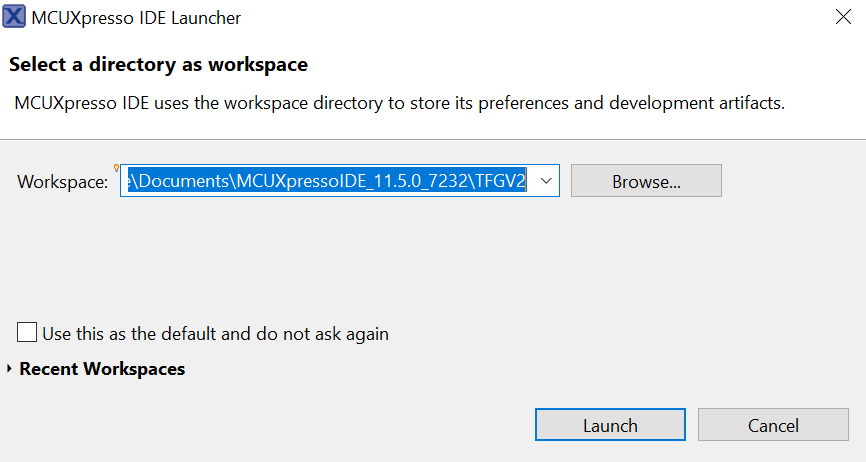
\includegraphics[width=0.6\textwidth]{rutaProyectoIde}
	\caption{Elección de la ruta para guardar los proyectos en local.}
\end{figure}
\FloatBarrier

Tras elegir la ruta y pulsar `Launch' encontraremos la siguiente interfaz:

\imagen{IntPrincMCUXpresso}{Interfaz principal MCUXpresso.}

Como se puede apreciar en la figura anterior, el IDE proporciona una interfaz semejante al IDE Eclipse.


\subsection{Descarga e instalación del SDK}
Tras esta instalación del IDE, deberemos realizar el segundo paso en el que descargaremos el SDK. Podemos descargarlo también desde la web de NXP \cite{DLSDK}, en esta pestaña deberemos elegir el SDK correspondiente a la placa y comprobar que la versión sea superior a la 2.0. \\
A la hora de descargar el SDK es recomendable seleccionar todos sus paquetes por si los necesitáramos para futuros proyecto pero en caso de que no queramos descargarlos ahora podremos elegir solo algunos y descargarlos a `posteriori' según los vayamos necesitando. Mínimo deberemos descargar FreeRTOS y CMSIS.

\imagen{sdk}{Pagina de descarga del SDK para la placa K64F.}

La descarga del SDK nos permite construir proyectos específicos para nuestra placa, permite además añadir los componentes necesarios según las funcionalidades del SE. Nos ofrece la posibilidad de descargar e instalar drivers, el tipo de sistema operativo o configurar el middleware. En nuestro caso deberemos seleccionar como mínimo el sistema operativo FreeRTOS y como drivers lwIP y ADC para la medición del sensor de temperatura y la lectura de los potenciómetros. Para poder elegir estos add-ons deberemos clicar donde se muestra en la Figura \ref{clickSDK}.

\begin{figure}[!h]
	\centering
	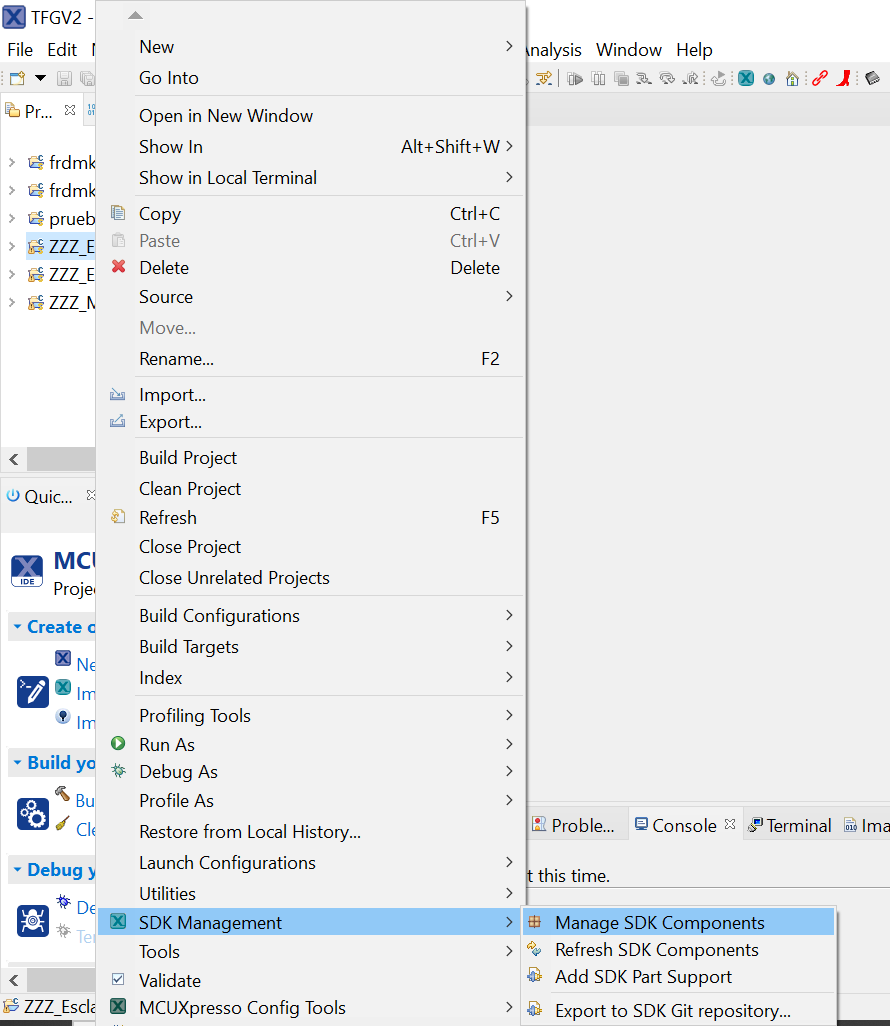
\includegraphics[width=0.6\textwidth]{GotoSDK}
	\caption{Abrir el SDK.}
	\label{clickSDK}
\end{figure}
\FloatBarrier

Posteriormente se abrirá un interfaz como la de la Figura \ref{UsingSDK}.

\imagen{UseSDK}{Elección de los Drivers necesarios.} \label{fig:UsingSDK}


Donde podremos elegir los componentes que queramos. Como se ve en la figura disponemos de un menú con distintas opciones: \extranjerismo{drivers, utilities, middleware.} Además la interfaz cuenta con una barra de buscador que nos facilita el trabajo.

\subsection{Importación del proyecto}
Importar un proyecto es bastante sencillo. Para ello iremos al repositorio de GitHub de este proyecto y descargamos los tres proyectos que componen el sistema en un `.zip'. Una vez descargados tan solo tendremos que pulsar en la opción 'import project from file system' que aparece en la Figura \ref{fig:import}:

\imagen{ImportacionProyecto}{Importación de un Proyecto.} \label{import}

Seleccionamos la ruta del proyecto o el archivo `.zip' y pulsamos en `finish'. De esta manera ya tendríamos el proyecto importado en nuestro IDE. En caso de hacerlo con el `.zip' nos saldrá otra pantalla más, en la que mi recomendación es que marquemos la opción de copiar el proyecto en la ruta de proyecto que elegimos previamente.

\subsection{ConfigTools: Configuración de pines, relojes y periféricos}
La configuración a bajo nivel de la placa es una de las partes más importantes y a la vez más complejas de entender al principio, por ello voy a explicar brevemente cómo funcionan estas interfaces del IDE.

\begin{description}
\item[Pines] Estas placas disponen de varios pines que son configurables permitiendo así la integración de varios periféricos y aumentando su funcionalidad. En la siguiente figura podemos observar la interfaz para configurarlo:

\imagen{PinesMCUX}{Interfaz de los Pines en MCUXpresso.}

En la parte izquierda de la figura vemos la lista de todos los pines que podemos configurar, que en el caso de esta placa son más de 100. Cada uno de estos pines tiene distintas configuraciones que podremos elegir según nuestras necesidades. \\ 
En la parte inferior nos muestra la lista de pines que ya hemos seleccionado y configurado. \\
Por último, en la parte de la derecha tenemos la imagen del controlador con todos sus pines. Los pines que ya se está utilizando aparecen remarcados en verde.
\item[Relojes] En el caso de este software se ha utilizado siempre el reloj configurado por defecto pero podemos configurar más relojes dependiendo del objetivo del periférico que vaya a usarlo. La Figura \ref{fig:relojes2} nos muestra una imagen de la interfaz.

\imagen{RelojesMCUX2}{Interfaz de la tabla de los Relojes en MCUXpresso.} \label{relojes2}

En la figura anterior se ven los relojes asignados a distintos elementos de la placa y en la parte izquierda los asignados a los periféricos. Estos relojes se pueden cambiar en un rango de frecuencias que se muestran en el diagrama de relojes de la Figura \ref{fig:relojes1}.
\imagen{RelojesMCUX}{Interfaz del diagrama de los relojes en MCUXpresso} \label{relojes1}

\item[Periféricos] el microcontrolador permite conectar varios periféricos a la placa al mismo tiempo. En la Figura \ref{fig:perifericos} se muestran cuales son:

\imagen{PerifericosMCUX}{Interfaz de los Periféricos en MCUXpresso.} \label{perifericos}

Como se puede apreciar, hay algunos repetidos como por ejemplo UART puesto que esta placa permite tener hasta 4 comunicaciones UART configurables al mismo tiempo. En algunas ocasiones, podría darse el caso de que no se puedan añadir más periféricos de esta lista porque los pines que son configurables para ese fin están siendo utilizados, aunque esto solo pasara en casos de sistemas SE muy concretos. \\
Cada una de las configuraciones de los periféricos tiene sus correspondientes opciones específicas. Estas configuraciones nos ayudan para que no tengamos que configurarlas programando y solo tengamos que hacer `click’ o elegir algunas de ellas. 
\end{description}

\section{Compilación, instalación y ejecución del proyecto}\label{sec:compilacion}

Una vez que hemos importado el proyecto, vamos a la carpeta sources y vemos que el fichero tiene los datos fuente del proyecto. Para poder compilar clicaremos en la opción \extranjerismo{build} para ver si el proyecto compila adecuadamente o tiene errores.

\begin{figure}[!h]
	\centering
	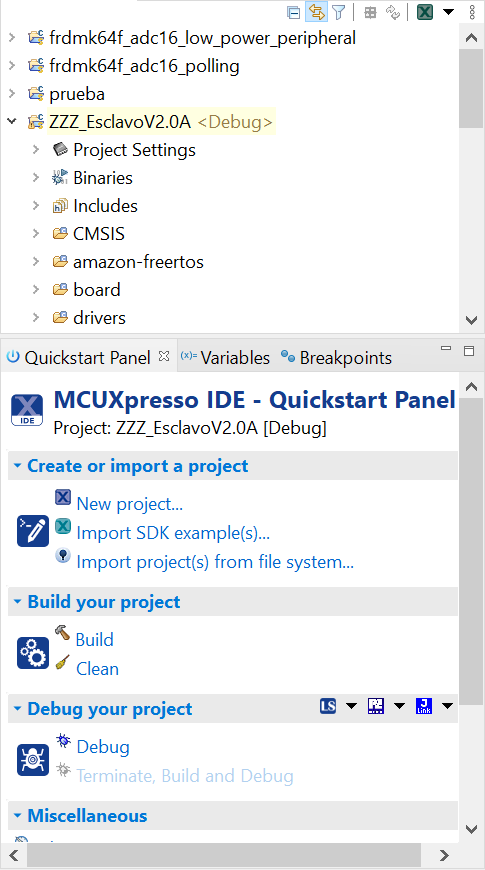
\includegraphics[width=0.5\textwidth]{compilacion}
	\caption{Compilación del Proyecto.}
\end{figure}
\FloatBarrier

Posteriormente deberemos conectar por USB la placa FRDM K64F al ordenador. Antes de seguir con el \extranjerismo{debugueo}, es importante que la placa esté en modo OpenSDA, para ello, si es la primera vez que la usamos, deberemos pulsar el botón reset mientras conectamos la placa al ordenador. Tras esto se debería de abrir una carpeta llamada `bootloader' donde deberemos copiar el fichero openSDA. Desconectamos y conectamos la placa de nuevo y la placa quedaría lista para realizar la escritura, o flash, de los archivos binarios del proyecto. 
Para este paso debemos pulsar la opción `debug' para iniciar la depuración. Una vez comience la ejecución se abrirá una consola y podremos utilizar el SE sin problemas. La primera vez que usemos una placa el IDE nos solicita la identificación de la misma. Para ello deberemos seleccionar el uso de `Segger J-Link Probes' que es compatible con OpenSDA y el adaptador serie y de depuración que viene integrado en la placa.

Dicho esto, es importante recalcar que estos métodos para compilar y depurar el programa no son los únicos, puesto que en el IDE se disponen de varios menús que en ocasiones repiten las mismas funcionalidades. Como dato a tener en cuenta, es interesante saber que la ejecución de la opción debug trae consigo la compilación del proyecto de manera automática si no se realizó manualmente antes de ejecutarse.

\section{Distribución de pines} \label{distribucionDePines}
En este apartado se muestran los pines usados para la comunicación de la pantalla LCD y de los motores. En la figura \ref{pinesUsados} se muestran los pines de la placa FRDM K64F.

\begin{figure}[!h]
	\centering
	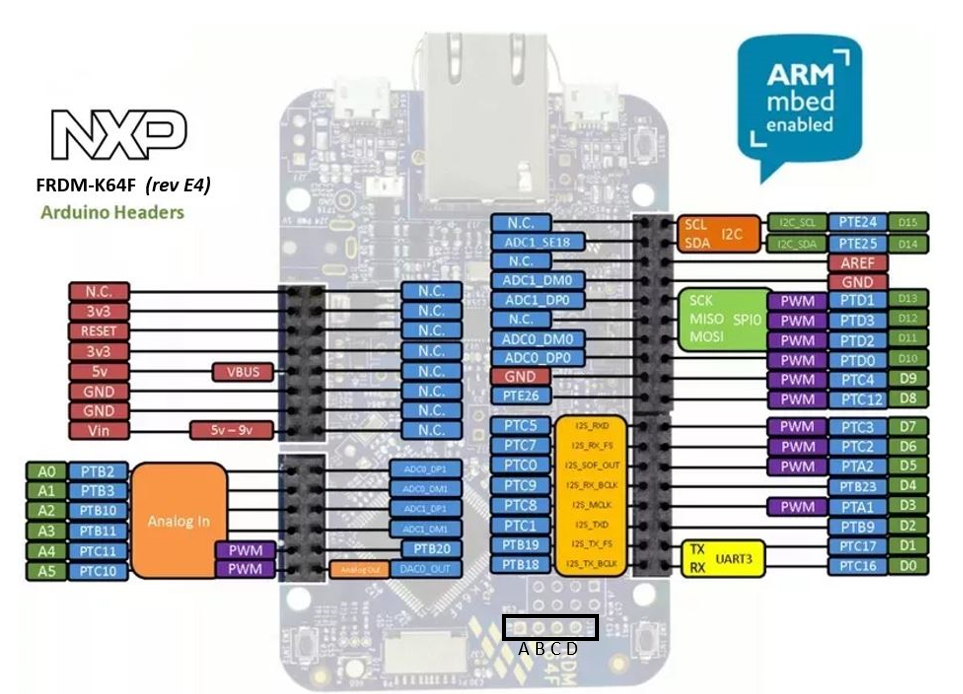
\includegraphics[width=0.9\textwidth]{pinesUsados}
	\caption{Definición de los pines de la placa FRDM K64F.}\label{pinesUsados}
\end{figure}

La figura \ref{ayudaPines} muestra las conexiones de la pantalla LCD y la placa controladora de los motores para poder entender mejor las siguientes tablas.

\begin{figure}[!h]
 \centering
  \subfloat[Módulo I2C LCD]{
    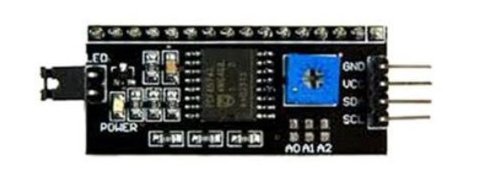
\includegraphics[width=0.5\textwidth]{moduloLCD.png}}
  \subfloat[Controladora MD25]{
    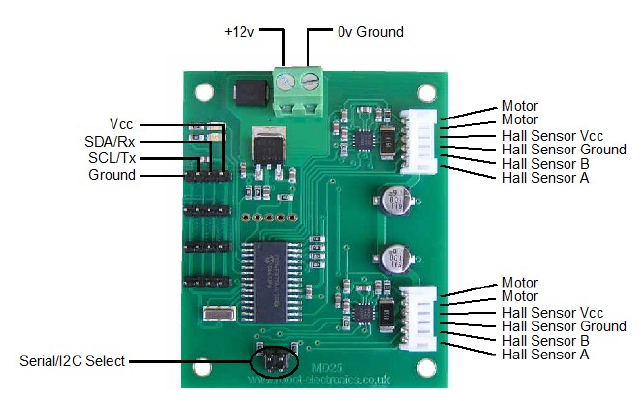
\includegraphics[width=0.5\textwidth]{placaMotor.png}}
 \caption{Conexión de Pines}\label{ayudaPines}
\end{figure}

\newpage

Los pines de la pantalla LCD se conectarán a los pines de la placa especificados en la tabla \ref{tabla:pinesLCD}\\

\tablaSmallSinColores{Pines FRDM K64F y pantalla LCD.}{c c}{pinesLCD}
{\multicolumn{1}{c}{ Pin K64F } & Pin Pantalla LCD\\}
{
PTE24 & SCL \\
PTE25 & SDA \\
5V & VCC \\
GND & TIERRA \\
}

En la parte inferior de la figura \ref{pinesUsados} hay cuatro pines marcados con las letras: A,B,C,D, a los que se conectaran a la placa controladora de los motores. En la tabla \ref{tabla:pinesMotor} se muestra su disposición.

\tablaSmallSinColores{Pines FRDM K64F y motores EMG30.}{c c}{pinesMotor}
{\multicolumn{1}{c}{ Pin K64F } & Pin Motor EMG30\\}
{
A: 3v & VCC \\
B: Tierra & GND \\
C: PTC14, UART, RX & TX \\
D: PTC15, UART, TX & RX \\
}

\section{Pruebas del sistema: Packet Sender}
Otra herramienta que puede ayudar enormemente a los desarrolladores es packet sender. Para descargarla tendremos que ir a su página web oficial \cite{DLPS} y descargar la herramienta para el sistema operativo donde vayamos a utilizarla. Packet Sender permite enviar paquetes por el protocolo tcp, a una ip y un puerto determinados. Además se pueden guardar nuestros propios comandos de envío para reutilizarlos de forma más sencilla. De esta forma, conseguimos poder comprobar si las placas reciben los comandos adecuadamente y cómo se comportan al recibirlo. Es como tener otra placa en red pero los comandos se envían de forma más sencilla desde nuestro propio ordenador.

\imagen{packetSender}{Interfaz de la herramienta Packet Sender.}



\apendice{Documentación de usuario} \label{ch:man-user}



\section{Introducción} \label{sec:man-user-intro}
Para que cualquier persona interesada pueda usar el sistema desarrollado,
este apéndice muestra los pasos necesarios.

Se indican los requisitos para la puesta en marcha del sistema empotrado
y de la aplicación web. También se indican las instrucciones para su correcta
instalación. Por último, un pequeño manual explica brevemente las funciones
accesibles desde la aplicación web.



\section{Requisitos de usuarios} \label{sec:man-user-req}
Como el sistema está compuesto por el sistema empotrado y por la aplicación web
es requisito fundamental tener ambos componentes listos para su utilización
por parte del usuario.


\subsection{Requisitos del sistema empotrado} \label{sec:man-user-req-se}
El sistema empotrado debe contar con el \sw{} almacenado en su memoria. En caso
de no estarlo, se deben seguir los pasos descritos en el apéndice con la
Documentación técnica de programación \ref{ch:man-dev}, en concreto, la sección
dedicada a la Compilación, escritura y ejecución del sistema empotrado
\ref{sec:exe-se}.


Para que el sistema empotrado pueda solicitar y recibir una dirección IP se
utiliza el protocolo DHCP. Por lo tanto, se requiere de la presencia de un
servidor DHCP en la red. Habitualmente, los \extranjerismo{routers} usados
en redes pequeñas de tipo residenciales o Small Offices/Home Offices (SOHO)
llevan incluido un servidor DHCP facilitando la instalación al usuario.


\subsection{Requisitos de la aplicación web} \label{sec:man-user-req-aw}
La aplicación web es accesible desde cualquier navegador web. Se puede usar
cualquiera de los dispositivos habituales usados para acceder a la web. Bien
sean equipos de sobremesa o dispositivos móviles.

Como la aplicación se ejecuta en un servidor de aplicaciones, es necesario
contar con uno en la misma red donde se conecta el sistema empotrado. Las
instrucciones sobre como desplegar la aplicación se detallan en el apéndice
con la Documentación técnica de programación \ref{ch:man-dev}, en concreto, la
sección dedicada a la Compilación, escritura y ejecución de la aplicación web
\ref{sec:exe-aw}.



\section{Instalación} \label{sec:man-user-inst}
Si se cumplen los requisitos anteriores, la instalación se reduce a conectar y
arrancar el sistema empotrado.

Para establecer la conexión a la red basta con un cable de par trenzado
conectado al sistema empotrado en un extremo y a un \extranjerismo{switch},
\extranjerismo{router} u otro dispositivo de acceso a la red en el
otro.

Para finalizar, el arranque del sistema empotrado se realiza automáticamente
cuando se conecta un cable USB en alguno de sus puertos Micro-USB. Esta conexión
se encarga de suministrar la alimentación eléctrica al sistema.

\imagenancho{boot}{Arranque del sistema empotrado}{!h}{0.6}

Una vez encendido, el sistema empotrado solicitará una dirección IP. Tras
obtenerla, la mostrará por pantalla junto al puerto TCP abierto.
Cuando se muestran estos datos ya es posible enviar instrucciones al sistema
empotrado desde la aplicación web.



\section{Manual del usuario} \label{sec:man-user}
La aplicación web está accesible desde la URL http://servidor:8080/web-app/,
siendo ``servidor'' la dirección del servidor de aplicaciones.

\imagenancho{landing}{Vista general de la web}{!h}{0.9}

Los botones de la barra de navegación permiten desplazarse directamente a las
funciones.

\imagenancho{navigation}{Barra de navegación}{!h}{0.75}

Para poder transmitir las instrucciones al sistema empotrado hay que indicar
los ajustes de red. Un texto provisional muestra un ejemplo del tipo de
direcciones habitual en redes locales y el puerto TCP usado durante el
desarrollo.

\imagenancho{network}{Ajustes de red sin establecer}{!h}{0.75}

Estos datos los proporciona el sistema empotrado tras su arranque. 

\imagenancho{dhcp}{IP y puerto del sistema empotrado}{!h}{0.6}

Tras escribir los datos, pulsando conectar la aplicación web queda preparada
para comunicarse con ese sistema empotrado.

\imagenancho{network2}{Ajustes de red establecidos}{!h}{0.75}

La primera función disponible es el encendido de las luces de colores usando
los LED RGB. El color de cada botón refleja el color de la luz a iluminar.
Por otro lado, pulsando el botón negro se apagan todos los LED encendidos.

\imagenancho{rgb}{Colores iluminables con los LED RGB}{!h}{0.75}

La segunda función muestra cadenas de caracteres en la pantalla LCD del sistema
empotrado. Para cada línea del LCD se proporciona un cuadro de texto diferente.
Cada cuadro se acompaña de un botón para confirmar el envío del mensaje.

\imagenancho{msg}{Envío de mensajes a la pantalla LCD}{!h}{0.75}

Por ejemplo, enviando el texto provisional que aparece por defecto la pantalla
del sistema empotrado muestra lo siguiente \footnote{Como el texto provisional
supera el límite de 16 caracteres del LCD, los últimos caracteres se descartan.}

\imagenancho{msg-lcd}{Mensajes enviados a la pantalla LCD}{!h}{0.6}

La tercera y última función disponible es la regulación de la intensidad del
brillo de unos LED mediante PWM. Para realizar esta regulación se muestran 
cuatro controles deslizantes de colores. Cada uno con el color del LED que
regula.

\imagenancho{pwm}{Controles deslizantes para los LED PWM}{!h}{0.8}

Todos los controles parten de la posición inicial de apagado (o 0\%).
Deslizándolos a derecha e izquierda se puede ajustar al valor que se quiera.

\imagenancho{pwm2}{Controles ajustados a diferentes valores}{H}{0.8}



% Genera la bibliografía.
\printbibliography

% Añade el aviso de la licencia.
\clearpage

\mbox{}
\vfill

\begin{figure}[!h]
  \centering
  
\includegraphics[width=0.2\textwidth]{ccbyncsa}
\end{figure}

\begin{center}
  Este obra está bajo una
  \href{https://creativecommons.org/licenses/by-nc-sa/4.0/}
    {licencia de Creative Commons Reconocimiento-NoComercial-CompartirIgual 4.0
    Internacional}.
\end{center}

\end{document}
